\documentclass[10pt,notheorems,xcolor=pdftex,dvipsnames,table]{beamer}
\usepackage[utf8]{inputenc}
\usefonttheme{serif}
\definecolor{light-gray}{gray}{0.95}
\setbeamercolor{background canvas}{bg=light-gray}
\linespread{1.2}
\usepackage[absolute,overlay]{textpos}
\usepackage{graphicx}
\usepackage{cancel}

\usepackage{calligra}

\usepackage{tikz}
\usetikzlibrary{decorations.pathreplacing}


\renewcommand{\{}{\left\lbrace}
\renewcommand{\}}{\right\rbrace}
\newcommand{\C}{\mathbb{C}}
\newcommand{\R}{\mathbb{R}}
\newcommand{\Z}{\mathbb{Z}}
\newcommand{\Q}{\mathbb{Q}}
\newcommand{\N}{\mathbb{N}}
\newcommand{\Gal}{\mathrm{Gal}}
\newcommand{\Aut}{\mathrm{Aut}}
\newcommand{\IN}{\mathrm{in}_{\leq}}
\newcommand{\lex}{\leq_{\mathrm{lex}}}
\newcommand{\lcm}{\mathrm{lcm}}
\newcommand{\wdots}[2]{ #1, \ldots ,#2 }
\renewcommand{\P}{\{ \wdots{p_1}{p_m} \}}
\newcommand{\K}{K[ \wdots{x_1}{x_n} ]}
\newcommand{\I}{\langle \wdots{p_1}{p_m}  \rangle}


\newtheorem{theorem}{Sætning}
\newtheorem{definition}{Definition}


\usepackage{array}
\usepackage{amsthm,amsmath,amssymb}
\usepackage{multirow}
\usepackage{multicol}
\usepackage{url}


\newcommand{\divides}{\bigm|}
\newcommand{\ndivides}{%
  \mathrel{\mkern.5mu % small adjustment
    % superimpose \nmid to \big|
    \ooalign{\hidewidth$\big|$\hidewidth\cr$\nmid$\cr}%
  }%
}


\begin{document}

\begin{frame}
	\frametitle{ \vspace*{1.5cm}
		\begin{center} 
			\Huge{Gröbner-baser} \linebreak \linebreak
			\normalsize{Bachelorforsvar ved Kristian \\
			Fredag d. 27. marts 2015}
		\end{center}}
		\begin{textblock*}{0.1cm}(8.78cm,7.78cm) % {block width} (coords)
			
\includegraphics[width=4cm]{disposition/d1.jpg}
		\end{textblock*}
\end{frame}


\begin{frame}[t]
	\frametitle{ 
		\LARGE{Disposition}}
			\begin{enumerate}
				\item<1-> Motivation og baggrund
					\tikz[remember picture] \node[coordinate,xshift=0.3cm, yshift=0.2cm] (n1) {};
				\item<1-> Idéerne kort fortalt				
				\item<1-> Division af polynomier
				\item<1-> Gröbner-baser
				\item<1-> Anvendelser
				\item<1-> Lyn-opsummering
					\tikz[remember picture] \node[coordinate, xshift=1.25cm, yshift=-0.1cm] (n2) {};
				\item<3->  Spørgsmål
			\end{enumerate}
				\visible<2->{
					\begin{tikzpicture}[overlay,remember picture]
						\draw[thick,decorate,decoration={brace,amplitude=7pt}]
				    	(n1) -- (n2) node[midway, right=10pt] {25 min.};
					\end{tikzpicture} 		} 
			\begin{textblock*}{0.1cm}(8.78cm,7.78cm) 
				
\includegraphics[width=4cm]{disposition/d11.jpg}
			\end{textblock*}
\end{frame}




	
\begin{frame}[t]
\frametitle{
		\LARGE{1. Motivation og baggrund}}
			\visible<1->{ Løsning af systemer af ikke-lineære polynomiumsligninger }
			\begin{textblock*}{0.1cm}(1.5cm,1.8cm) 
				\visible<2->{ \begin{align*}
					x^2+y^2+z^2-1 &= 0,  \\
					x+y+z         &= 0,  \\
					y-3z 		  &= 0.
				\end{align*}}
			\end{textblock*}
			\begin{textblock*}{0.1cm}(7cm,2.2cm)  
				\visible<3->{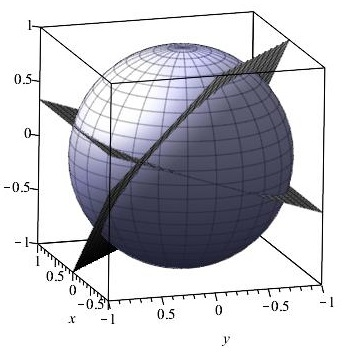
\includegraphics[scale=0.4]{ex1.jpg} }
			\end{textblock*}
			\begin{textblock*}{3cm}(2.2cm,4.5cm)
				\visible<4->{ {\color{blue} $\downarrow$ \emph{Gröbner basen} } } 
			\end{textblock*}
			\begin{textblock*}{0.1cm}(2.6cm,4.6cm)
				\visible<4->{ \begin{align*}
					26z^2-1       &= 0,  \\
					y-3z          &= 0,  \\
					x+y+z 		  &= 0.
				\end{align*} }
			\end{textblock*}
			\begin{textblock*}{0.1cm}(8.78cm,7.78cm)  
				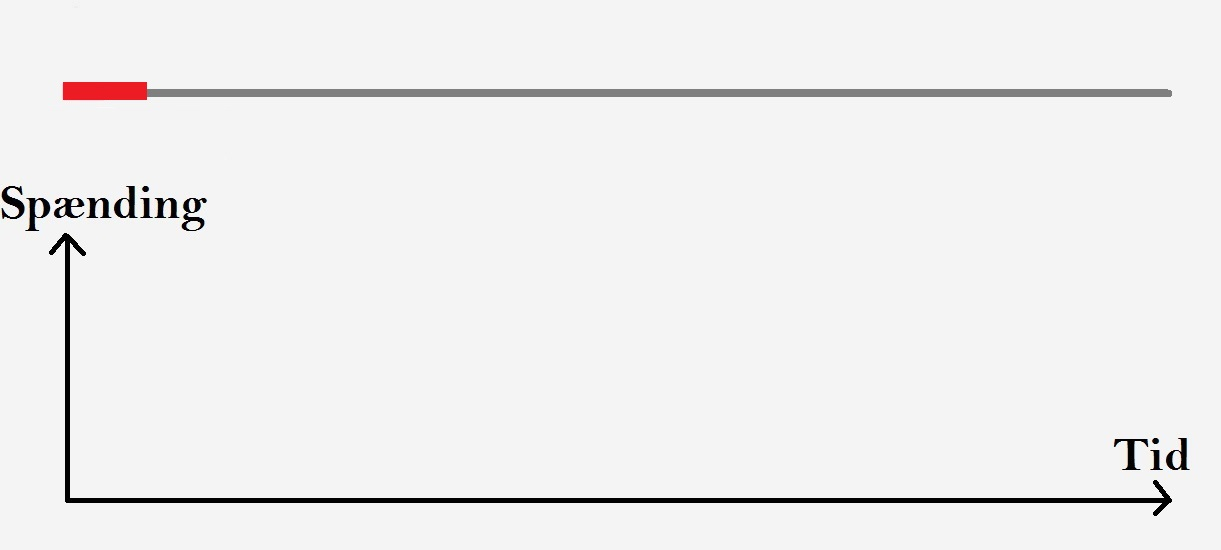
\includegraphics[width=4cm]{disposition/d4.jpg}
			\end{textblock*}
\end{frame}

\begin{frame}[t]
\frametitle{
		\LARGE{1. Motivation og baggrund}}
			\visible<1->{ Løsning af systemer af ikke-lineære polynomiumsligninger }
			\begin{textblock*}{0.1cm}(1.5cm,1.8cm) 
				\visible<1->{ \begin{align*}
					x^2+y^2+z^2-1 &= 0,  \\
					x+y+z         &= 0,  \\
					y-3z 		  &= 0.
				\end{align*}}
			\end{textblock*}
			\begin{textblock*}{0.1cm}(7cm,2.2cm)  
				\visible<1->{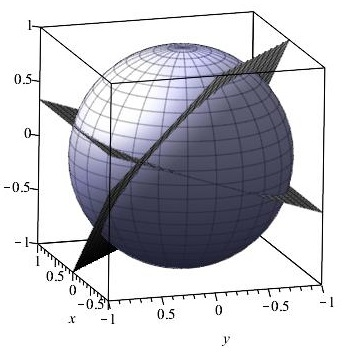
\includegraphics[scale=0.4]{ex1.jpg} }
			\end{textblock*}
			\begin{textblock*}{3cm}(2.2cm,4.5cm)
				\visible<1->{ {\color{blue} $\downarrow$ \emph{Gröbner basen} } } 
			\end{textblock*}
			\begin{textblock*}{0.1cm}(2.6cm,4.6cm)
				\visible<1->{ \begin{align*}
					26z^2-1       &= 0,  \\
					y-3z          &= 0,  \\
					x+y+z 		  &= 0.
				\end{align*} }
			\end{textblock*}
			\begin{textblock*}{6cm}(1.8cm,7.8cm)
				\visible<1->{ \large{ \calligra{God gammeldags Algebra}} }
			\end{textblock*}
			\begin{textblock*}{0.1cm}(8.78cm,7.78cm)  
				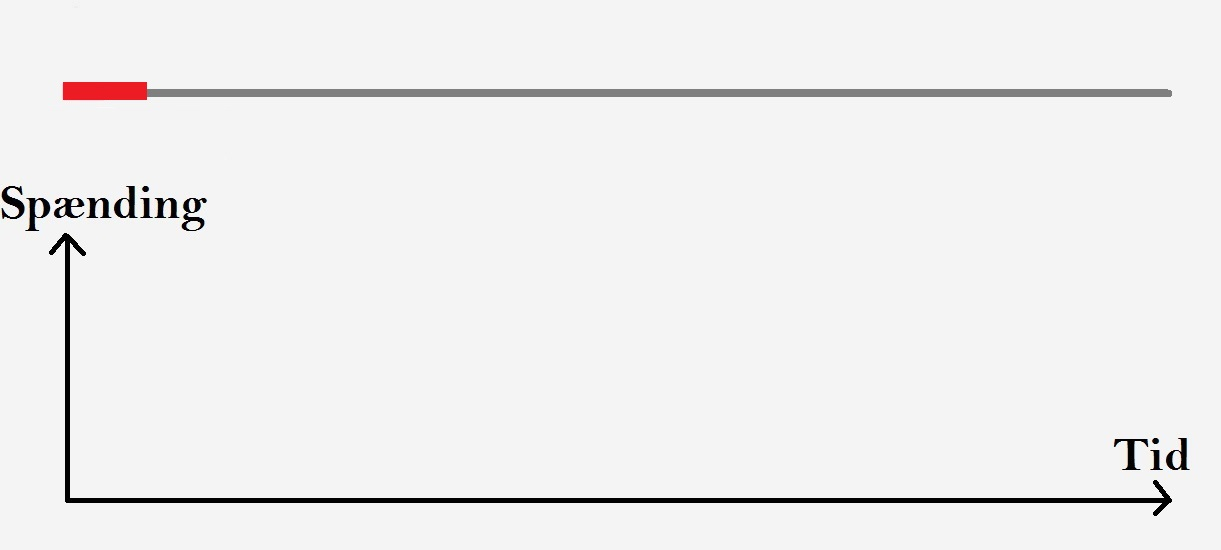
\includegraphics[width=4cm]{disposition/d4.jpg}
			\end{textblock*}
\end{frame}

\begin{frame}[t]
\frametitle{
		\LARGE{1. Motivation og baggrund}}
			\visible<1->{ Løsning af systemer af ikke-lineære polynomiumsligninger }
			\begin{textblock*}{0.1cm}(1.5cm,1.8cm) 
				\visible<1->{ \begin{align*}
					x^2+y^2+z^2-1 &= 0,  \\
					x+y+z         &= 0,  \\
					y-3z 		  &= 0.
				\end{align*}}
			\end{textblock*}
			\begin{textblock*}{0.1cm}(7cm,2.2cm)  
				\visible<1->{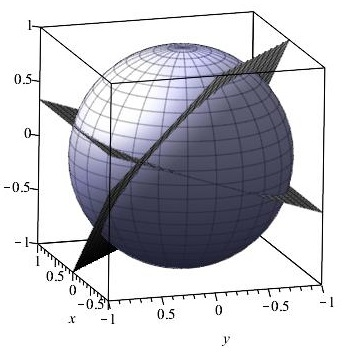
\includegraphics[scale=0.4]{ex1.jpg} }
			\end{textblock*}
			\begin{textblock*}{3cm}(2.2cm,4.5cm)
				\visible<1->{ {\color{blue} $\downarrow$ \emph{Gröbner basen} } } 
			\end{textblock*}
			\begin{textblock*}{0.1cm}(2.6cm,4.6cm)
				\visible<1->{ \begin{align*}
					26z^2-1       &= 0,  \\
					y-3z          &= 0,  \\
					x+y+z 		  &= 0.
				\end{align*} }
			\end{textblock*}
			\begin{textblock*}{6cm}(1.8cm,7.8cm)
				\visible<1->{ \large{ \calligra{God \cancel{gammeldags} Algebra}} }
			\end{textblock*}
			\begin{textblock*}{0.1cm}(8.78cm,7.78cm)  
				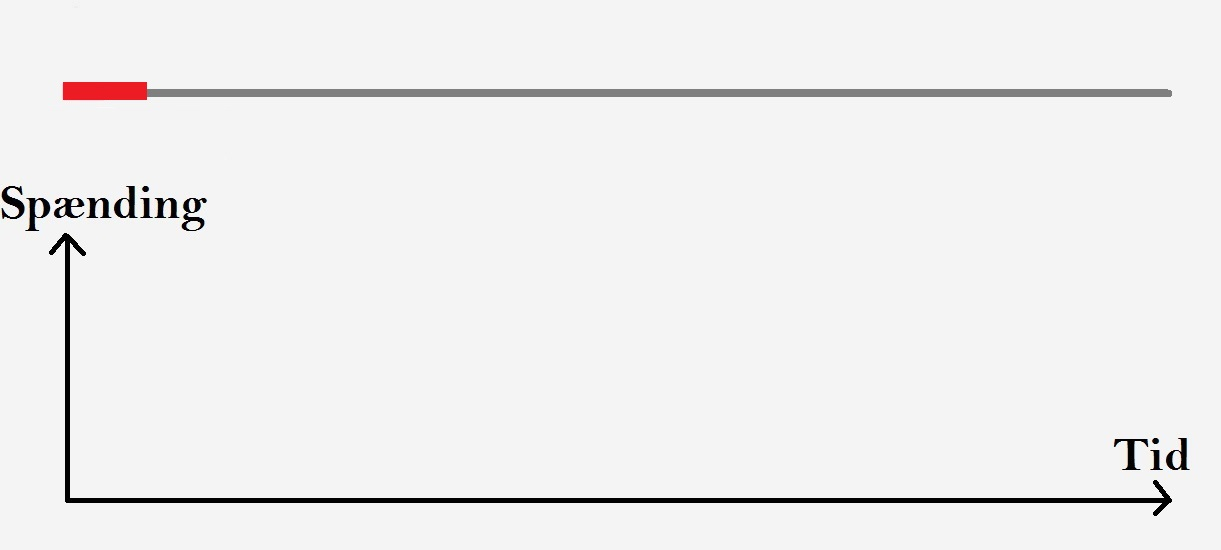
\includegraphics[width=4cm]{disposition/d4.jpg}
			\end{textblock*}
\end{frame}




\begin{frame}[t]
\frametitle{
		\LARGE{1. Motivation og baggrund}}
			\begin{textblock*}{0.1cm}(1cm,1.5cm)
				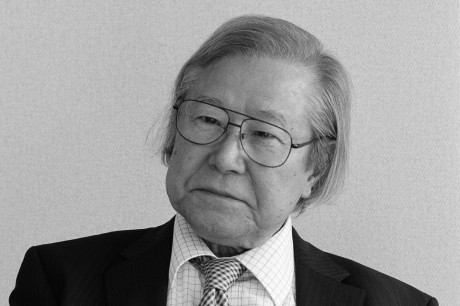
\includegraphics[scale=0.3]{hironaka.jpg}
			\end{textblock*}
			\begin{textblock*}{3cm}(2.2cm,5cm)
				Hironaka (1931 -)
			\end{textblock*}
			\begin{textblock*}{0.1cm}(6.5cm,1.5cm)
				\visible<1->{
\includegraphics[scale=0.51]{buchberger.jpg}  }
			\end{textblock*}
			\begin{textblock*}{4cm}(7.2cm,5cm)
				\visible<1->{Buchberger (1942 -)}
			\end{textblock*}
			\begin{textblock*}{0.1cm}(5cm,5.5cm)
				\visible<2->{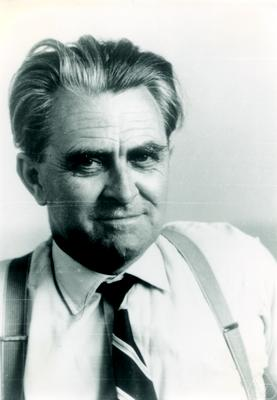
\includegraphics[scale=0.22]{groebner.jpg}  }
			\end{textblock*}
			\begin{textblock*}{4cm}(4.3cm,8.8cm)
				\visible<2->{Gröbner (1899 - 1980)}
			\end{textblock*}
			\begin{textblock*}{0.1cm}(8.78cm,7.78cm)  
				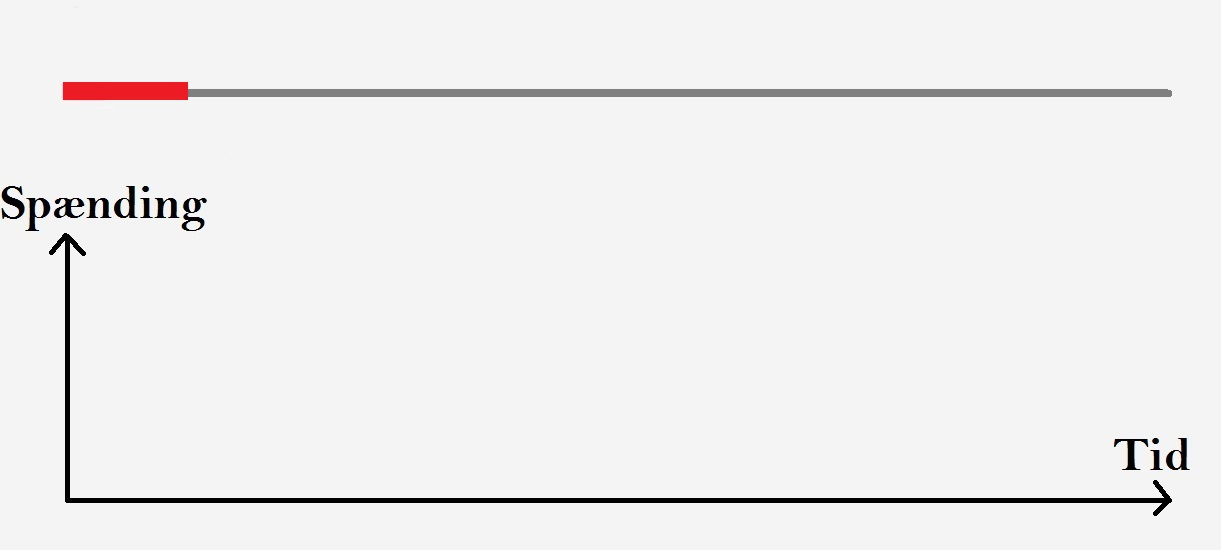
\includegraphics[width=4cm]{disposition/d5.jpg}
			\end{textblock*}
\end{frame}










\begin{frame}[t]
\frametitle{
		\LARGE{2. Idéerne kort fortalt}}
			Givet \hspace*{1.8cm} i $\K$
			\begin{textblock*}{0.1cm}(2.2cm,0.9cm)
						\begin{align*}
							p_1 &= 0, \\
							p_2 &= 0, \\
							&\vdots \\
							p_m &= 0.
						\end{align*}
			\end{textblock*} 
			\begin{textblock*}{4cm}(1.5cm,4.7cm)
				\visible<2->{ $I = \I$,}
			\end{textblock*}
			\begin{textblock*}{6cm}(4.5cm,4.7cm)
				\visible<2->{ ${\color{gray}p \in I \Leftrightarrow p = a_1p_1 + \cdots + a_mp_m} $}
			\end{textblock*}
			\begin{textblock*}{4cm}(3.5cm,5.7cm)
				\visible<3->{ ${\color{blue}P = \{p_1,\ldots ,p_s\} } \subseteq I$}
			\end{textblock*}
			%\begin{textblock*}{4cm}(5.5cm,5.7cm)
			%	\visible<4>{ ``${\color{blue}p_i} \neq a\cdot {\color{blue} p_j}$'', for $i\neq j$}
			%\end{textblock*}
			\begin{textblock*}{7cm}(3.5cm,6.5cm)
				\visible<4->{ For ethvert $p \in I$ skal findes ${\color{blue}p_i \in P}$ så ``${\color{blue}p_i}\cdot a = p$''}
			\begin{textblock*}{4cm}(3.5cm,7,9cm)
				\visible<5->{$S$-polynomiet.}
			\end{textblock*}
			\end{textblock*}
			\begin{textblock*}{0.1cm}(8.78cm,7.78cm)  
				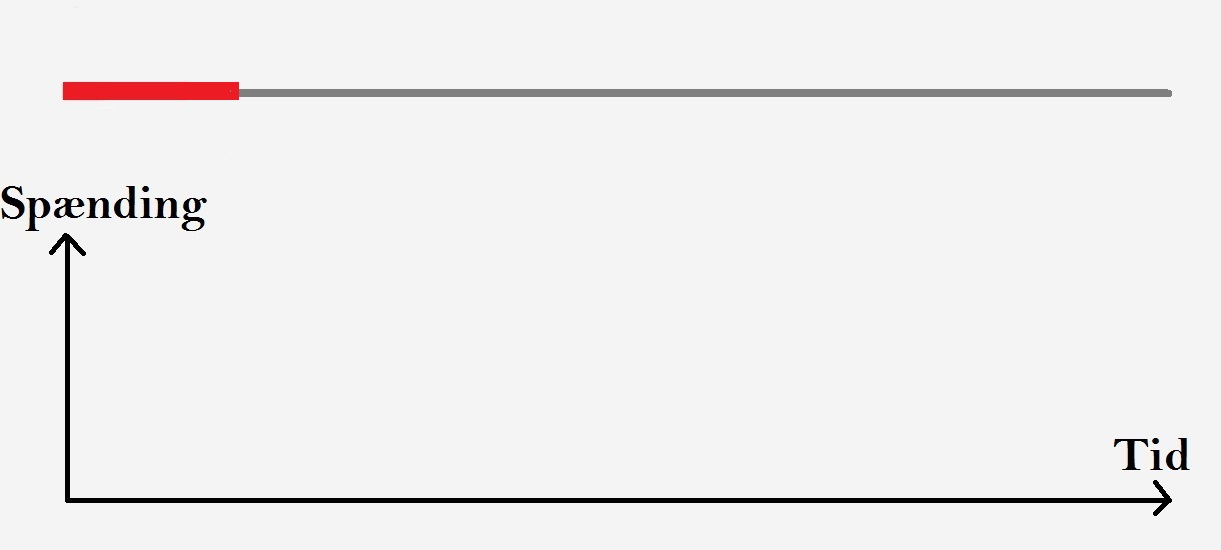
\includegraphics[width=4cm]{disposition/d6.jpg}
			\end{textblock*}
\end{frame}


%\begin{frame}[t]
%\frametitle{
%		\LARGE{3. Division af polynomier}}
% 			\begin{textblock*}{1cm}(2.2cm,0.9cm)
%				\visible<1>{\begin{align*}
%					{\color{red}3x^4}+3x^2+5\ :\ {\color{red}x^2}-2\ =
%				\end{align*}}
%			\end{textblock*} 
%			\begin{textblock*}{1cm}(2.2cm,0.9cm)
%				\visible<2>{\begin{align*}
%					{\color{red}3x^4}+3x^2+5\ :\ {\color{red}x^2}-2\ =\ 3x^2 
%				\end{align*}}
%			\end{textblock*} 
%			\begin{textblock*}{1cm}(2.2cm,0.9cm)
%				\visible<3>{\begin{align*}
%					&{\color{red}3x^4}+3x^2+5\ :\ {\color{red}x^2}-2\ =\ 3x^2  \\
%					&\underline{3x^4-6x^2} 
%				\end{align*}}
%			\end{textblock*} 
%			\begin{textblock*}{1cm}(2.2cm,0.9cm)
%				\visible<4>{\begin{align*}
%					&3x^4+3x^2+5\ :\ {\color{red}x^2}-2\ =\ 3x^2  \\
%					&\underline{3x^4-6x^2} \\
%					&\hspace*{0.9cm} {\color{red}9x^2}+5  
%				\end{align*}}
%			\end{textblock*} 
%			\begin{textblock*}{1cm}(2.2cm,0.9cm)
%				\visible<5>{\begin{align*}
%					&3x^4+3x^2+5\ :\ {\color{red}x^2}-2\ =\ 3x^2 + 9  \\
%					&\underline{3x^4-6x^2} \\
%					&\hspace*{0.9cm} {\color{red}9x^2}+5  
%				\end{align*}}
%			\end{textblock*} 
%			\begin{textblock*}{1cm}(2.2cm,0.9cm)
%				\visible<6>{\begin{align*}
%					&3x^4+3x^2+5\ :\ {\color{red}x^2}-2\ =\ 3x^2 + 9  \\
%					&\underline{3x^4-6x^2} \\
%					&\hspace*{0.9cm} 9x^2+5  \\
%					&\hspace*{0.9cm} \underline{9x^2-18}
%				\end{align*}}
%			\end{textblock*} 
%			\begin{textblock*}{1cm}(2.2cm,0.9cm)
%				\visible<7>{\begin{align*}
%					&3x^4+3x^2+5\ :\ {\color{red}x^2}-2\ =\ 3x^2 + 9  \\
%					&\underline{3x^4-6x^2} \\
%					&\hspace*{0.9cm} 9x^2+5  \\
%					&\hspace*{0.9cm} \underline{9x^2-18} \\
%					&\hspace*{1.8cm} {\color{red}23} 
%				\end{align*}}
%			\end{textblock*}
%			\begin{textblock*}{1cm}(2.2cm,0.9cm)
%				\visible<8>{\begin{align*}
%					&3x^4+3x^2+5\ :\ {\color{red}x^2}-2\ =\ 3x^2 + 9  \\
%					&\underline{3x^4-6x^2} \\
%					&\hspace*{0.9cm} 9x^2+5  \\
%					&\hspace*{0.9cm} \underline{9x^2-18} \\
%					&\hspace*{1.8cm} \underline{{\color{red}23}} \longrightarrow 23 \\
%					&\hspace*{2cm}  0. 
%				\end{align*}}
%			\end{textblock*}
%			\begin{textblock*}{1cm}(2.2cm,0.9cm)
%				\visible<9>{\begin{align*}
%					&3x^4+3x^2+5\ :\ {\color{red}x^2}-2\ =\ 3x^2 + 9  \\
%					&\underline{3x^4-6x^2} \\
%					&\hspace*{0.9cm} 9x^2+5  \\
%					&\hspace*{0.9cm} \underline{9x^2-18} \\
%					&\hspace*{1.8cm} \underline{{\color{red}23}} \longrightarrow 23 \\
%					&\hspace*{2cm}  0. 
%				\end{align*}}
%			\end{textblock*}
%			\begin{textblock*}{6cm}(2cm,5.5cm)
%				\visible<9> {Dvs. $3x^4+3x^2+5 = (x^2-2)(3x^2+9) + 23$.  }
%			\end{textblock*}
%			\begin{textblock*}{1cm}(2.2cm,0.9cm)
%				\visible<10>{\begin{align*}
%					&3x^4+3x^2+5\ :\ {\color{red}x^2}-2\ =\ 3x^2 + 9  \\
%					&\underline{3x^4-6x^2} \\
%					&\hspace*{0.9cm} 9x^2+5  \\
%					&\hspace*{0.9cm} \underline{9x^2-18} \\
%					&\hspace*{1.8cm} \underline{{\color{red}23}} \longrightarrow 23 \\
%					&\hspace*{2cm}  0. 
%				\end{align*}}
%			\end{textblock*}
%			\begin{textblock*}{6cm}(2cm,5.5cm)
%				\visible<10>{Dvs. $3x^4+3x^2+5 = (x^2-2)(3x^2+9) + 23$.  }
%			\end{textblock*}
%						\begin{textblock*}{7cm}(2cm,7cm)
%				\visible<10>{Bemærk, at $x^2 \nmid 23$  samt\\ $\deg(x^2\cdot 3x^2)\leq \deg(3x^4)$  }
%			\end{textblock*}
%\end{frame}

\begin{frame}[t]
	\frametitle{
		\LARGE{3. Division af polynomier}}
			\begin{textblock*}{1cm}(2.2cm,0.9cm)
				\visible<1>{\begin{align*}
					xy^4+3x^4+5\ :\ x^2-2y^2\ =\ ?
				\end{align*}}
			\end{textblock*}
				\visible<2->{ Vi har brug for det \emph{betydende led} (eng.: initial term)}
				\visible<3->{\begin{definition}[\bfseries{Betydende led}]
				Lad $p \in \K$ være givet ved
				\begin{align*}
					p = \sum_{v \in \N_0^n} a_vX^v.
				\end{align*}
				Lad desuden $u = \max_{\leq}\{v \in \N_0^n \mid a_v \neq 0 \}$. Det betydende led i polynomiet $p$ er
				\begin{align*}
					\IN(p) = a_up^u.
				\end{align*}
				\end{definition} }
			\begin{textblock*}{0.1cm}(8.78cm,7.78cm)  
				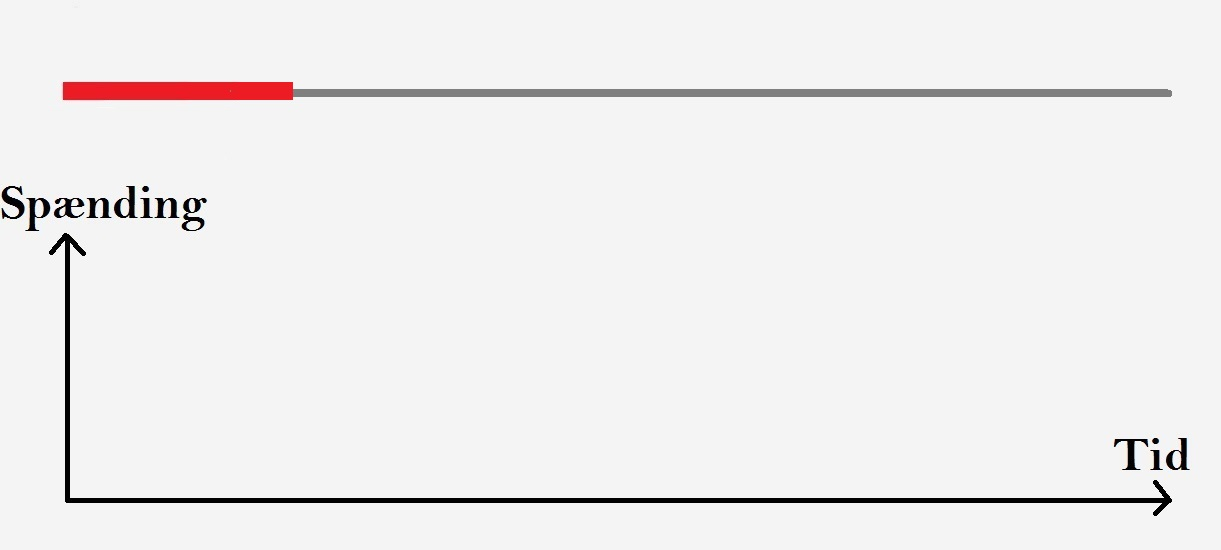
\includegraphics[width=4cm]{disposition/d7.jpg}
			\end{textblock*}
\end{frame}


\begin{frame}[t]
\frametitle{
		\LARGE{3. Division af polynomier}}
		\visible<1->{Vi har brug for en \emph{ledordning} (eng.: term ordering). \\} 
		\visible<2->{ Ex. på en ledordning:
		\begin{definition}[\bfseries{Lexicografiske ordning}]
						
					\end{definition} }
			\begin{textblock*}{0.1cm}(8.78cm,7.78cm)  
				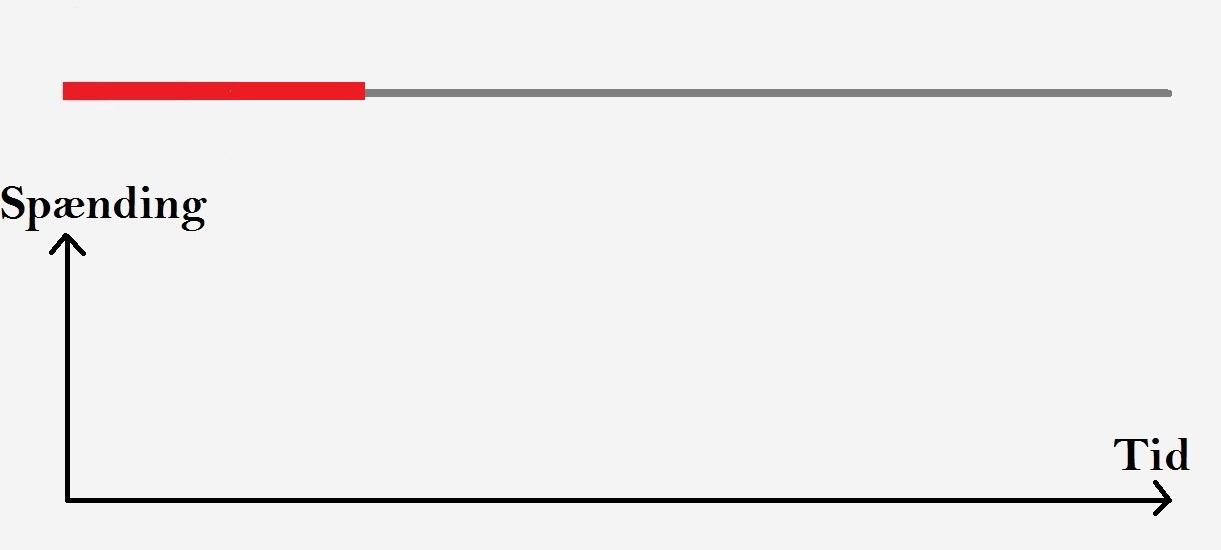
\includegraphics[width=4cm]{disposition/d8.jpg}
			\end{textblock*}
\end{frame}


\begin{frame}[t]
\frametitle{
		\LARGE{3. Division af polynomier}}
		\visible<1->{Vi har brug for en \emph{ledordning} (eng.: term ordering). \\} 
		\visible<1->{ Ex. på en ledordning:
		\begin{definition}[\bfseries{Lexicografiske ordning}]
		Lad $x = (x_1,\ldots ,x_n) \in \N_0^n$ og $y = (y_1,\ldots ,y_n) \in \N_0^n$.
					\begin{align*}
		x \lex y \quad  \Leftrightarrow \quad  &x_1 < y_1\  \text{eller} \\
		{\color{blue}x \leq y }\qquad \qquad \				   &x_1 = y_1\  \text{og}\  x_2 < y_2\  \text{eller}  \\
											   &x_1 = y_1\  \text{og}\  x_2 = y_2\  \text{og}\ x_3 < y_3\  \text{eller}  \\
											   & \qquad \vdots  \\
											   &x_1 = y_1\  \text{og}\  x_2 = y_2\  \text{og}\ \ldots\ \text{og}\  x_n = y_n.
						\end{align*}
					\end{definition} }
			\begin{textblock*}{0.1cm}(8.78cm,7.78cm)  
				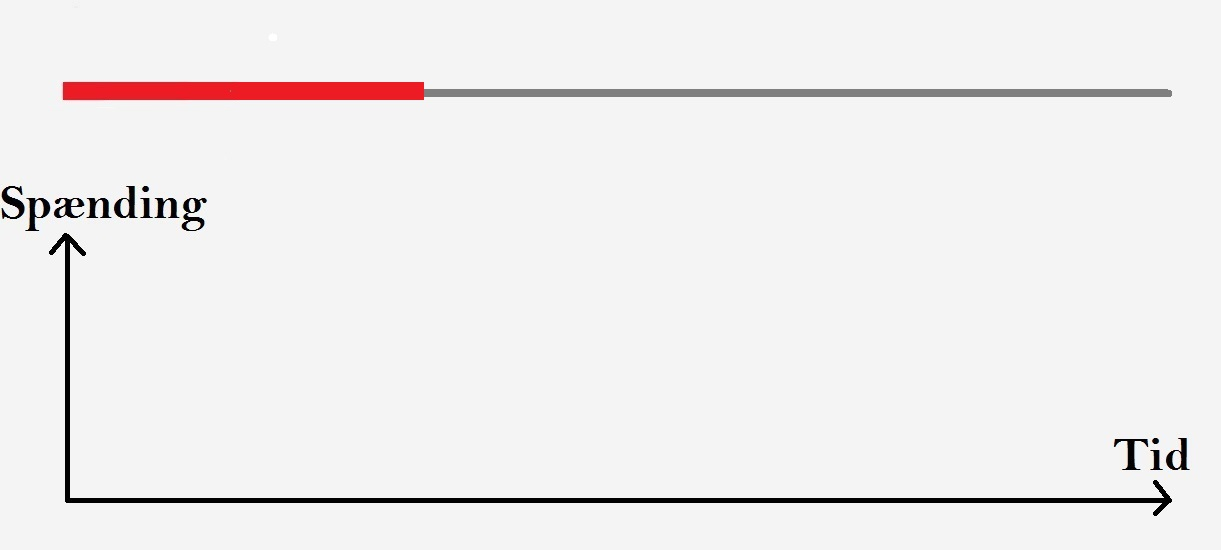
\includegraphics[width=4cm]{disposition/d9.jpg}
			\end{textblock*}
\end{frame}


\begin{frame}[t]
\frametitle{
		\LARGE{3. Division af polynomier}}
\begin{textblock*}{1cm}(2.2cm,0.9cm)
	\visible<1>{\begin{align*}
		&{\color{red}x^3y^2} + xy + z \ : \ \{{\color{red}x^2y} + 2\ ,\  {\color{red}x} + z \} \ = \ \{ \ ,\  \}.  
	\end{align*}}
\end{textblock*}
\begin{textblock*}{1cm}(2.2cm,0.9cm)
	\visible<2>{\begin{align*}
		&{\color{red}x^3y^2} + xy + z \ : \ \{{\color{red}x^2y} + 2\ ,\  {\color{red}x} + z \} \ = \ \{ xy\ ,\ \}.  \\
		& \underline{x^3y^2 + 2xy}
	\end{align*}}
\end{textblock*}
\begin{textblock*}{1cm}(2.2cm,0.9cm)
	\visible<3>{\begin{align*}
		&x^3y^2 + xy + z \ : \ \{{\color{red}x^2y} + 2\ ,\  {\color{red}x} + z \} \ = \ \{ xy\ ,\  \}.  \\
		& \underline{x^3y^2 + 2xy} \\
		& \hspace*{0.9cm}  {\color{red}-xy} + z  
	\end{align*}}
\end{textblock*}
\begin{textblock*}{1cm}(2.2cm,0.9cm)
	\visible<4>{\begin{align*}
		&x^3y^2 + xy + z \ : \ \{{\color{red}x^2y} + 2\ ,\  {\color{red}x} + z \} \ = \ \{ xy\ ,\ -y \}.  \\
		& \underline{x^3y^2 + 2xy} \\
		& \hspace*{0.9cm}  {\color{red}-xy} + z  \\
		& \hspace*{0.9cm}  \underline{-xy - yz} 
	\end{align*}}
\end{textblock*}
\begin{textblock*}{1cm}(2.2cm,0.9cm)
	\visible<5>{\begin{align*}
		&x^3y^2 + xy + z \ : \ \{{\color{red}x^2y} + 2\ ,\  {\color{red}x} + z \} \ = \ \{ xy\ ,\ -y \}.  \\
		& \underline{x^3y^2 + 2xy} \\
		& \hspace*{0.9cm}  {-xy + z}  \\
		& \hspace*{0.9cm}  \underline{-xy - yz} \\
		& \hspace*{1.9cm}  \underline{{ \color{red}yz} + z}  
	\end{align*}}
\end{textblock*}
\begin{textblock*}{1cm}(2.2cm,0.9cm)
	\visible<6>{\begin{align*}
		&x^3y^2 + xy + z \ : \ \{{\color{red}x^2y} + 2\ ,\  {\color{red}x} + z \} \ = \ \{ xy\ ,\ -y \}.  \\
		& \underline{x^3y^2 + 2xy} \\
		& \hspace*{0.9cm}  {-xy + z}  \\
		& \hspace*{0.9cm}  \underline{-xy - yz} \\
		& \hspace*{1.9cm}  \underline{{ \color{red}yz} + z} \longrightarrow yz  
	\end{align*}}
\end{textblock*}
\begin{textblock*}{1cm}(2.2cm,0.9cm)
	\visible<7>{\begin{align*}
		&x^3y^2 + xy + z \ : \ \{{\color{red}x^2y} + 2\ ,\  {\color{red}x} + z \} \ = \ \{ xy\ ,\ -y \}.  \\
		& \underline{x^3y^2 + 2xy} \\
		& \hspace*{0.9cm}  {-xy + z}  \\
		& \hspace*{0.9cm}  \underline{-xy - yz} \\
		& \hspace*{1.9cm}  \underline{yz + z} \longrightarrow yz  \\
		& \hspace*{2.7cm}  \underline{ {\color{red} z} } 
	\end{align*}}
\end{textblock*}
\begin{textblock*}{1cm}(2.2cm,0.9cm)
	\visible<8>{\begin{align*}
		&x^3y^2 + xy + z \ : \ \{{\color{red}x^2y} + 2\ ,\  {\color{red}x} + z \} \ = \ \{ xy\ ,\ -y \}.  \\
		& \underline{x^3y^2 + 2xy} \\
		& \hspace*{0.9cm}  {-xy + z}  \\
		& \hspace*{0.9cm}  \underline{-xy - yz} \\
		& \hspace*{1.9cm}  \underline{yz + z} \longrightarrow yz  \\
		& \hspace*{2.7cm}  \underline{ {\color{red} z} } \longrightarrow yz + z  
	\end{align*}}
\end{textblock*}
\begin{textblock*}{6cm}(2.2cm,0.9cm)
	\visible<9->{\begin{align*}
		&x^3y^2 + xy + z \ : \ \{{\color{red}x^2y} + 2\ ,\  {\color{red}x} + z \} \ = \ \{ xy\ ,\ -y \}.  \\
		& \underline{x^3y^2 + 2xy} \\
		& \hspace*{0.9cm}  {-xy + z}  \\
		& \hspace*{0.9cm}  \underline{-xy - yz} \\
		& \hspace*{1.9cm}  \underline{yz + z} \longrightarrow yz  \\
		& \hspace*{2.7cm}  \underline{ {\color{red} z} } \longrightarrow yz + z  \\
		& \hspace*{2.7cm}  0.  
	\end{align*}}
	\visible<10->{ Dvs.}
\end{textblock*}
\begin{textblock*}{8cm}(2.2cm,6cm)
	\visible<10->{\begin{align*}
		p = x^3y^2 + xy + z   =  \overbrace{xy(x^2y+2)}^{a_1p_1} + \overbrace{-y(x+z)}^{a_2p_2} + \overbrace{yz + z}^r.
	\end{align*}}
\end{textblock*}
			\begin{textblock*}{0.1cm}(8.78cm,7.78cm)  
				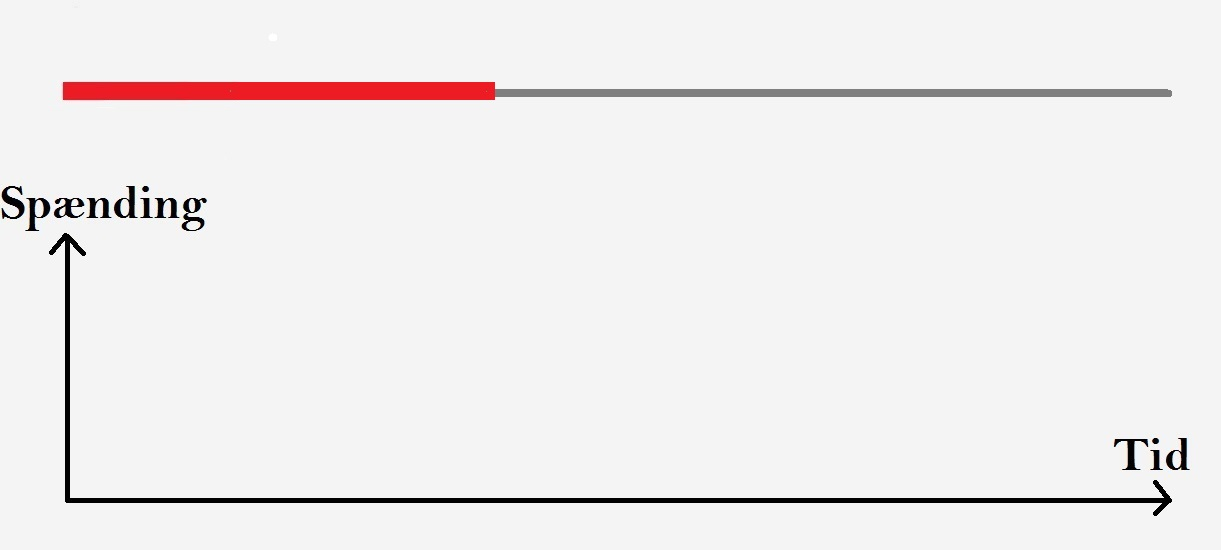
\includegraphics[width=4cm]{disposition/d10.jpg}
			\end{textblock*}
\end{frame}



\begin{frame}[t]
\frametitle{
		\LARGE{3. Division af polynomier}}
\begin{textblock*}{8cm}(2.2cm,1.5cm)
	\visible<1->{\begin{align*}
		p = x^3y^2 + xy + z   =  \overbrace{xy(x^2y+2)}^{a_1p_1} + \overbrace{-y(x+z)}^{a_2p_2} + \overbrace{yz + z}^r.
	\end{align*}}
	\visible<2->{ Bemærk, at $\IN(p_1) \nmid yz$ og $\IN(p_1) \nmid z$} \\
	\visible<3->{ \hspace*{2.05cm} $\IN(p_2) \nmid yz$ og $\IN(p_2) \nmid z$ }
\end{textblock*}
\begin{textblock*}{8cm}(2.2cm,5cm)
	\visible<4->{Hvis $P = \{p_1 , p_2\}$, så skriver vi $r = p^P$  }
\end{textblock*}
			\begin{textblock*}{0.1cm}(8.78cm,7.78cm)  
				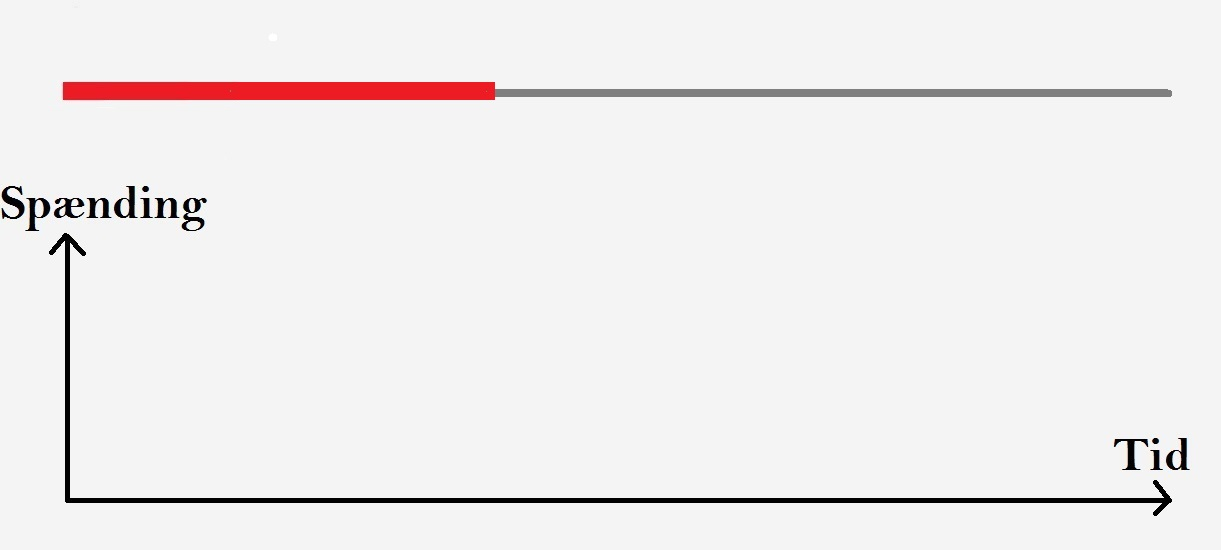
\includegraphics[width=4cm]{disposition/d10.jpg}
			\end{textblock*}
\end{frame}










\begin{frame}[t]
\frametitle{
		\LARGE{4. Gröbner-baser}}
	\visible<1->{\begin{definition}[\bfseries{Gröbner-basis}]
		Lad $P =\P \subseteq \K \setminus \{0\}$. Vi har, at $P$ er en Gröbner-basis for et ideal $I$ mht. en ledordning $\leq$, hvis
		\begin{itemize}
			\item[$G1$] $P \subseteq I$ og
			\item[$G2$] hvis der for alle $p \in I$ eksisterer et $p_i \in \P$ sådan, at $\IN(p_i) \mid \IN(p)$.
		\end{itemize}
	\end{definition}}
	\visible<2->{Hvis intet andet er givet, da er $I = \I$.  }\\
	\visible<3->{Lad os se et eksempel på en Gröbner-basis!}
			\begin{textblock*}{0.1cm}(8.78cm,7.78cm)  
				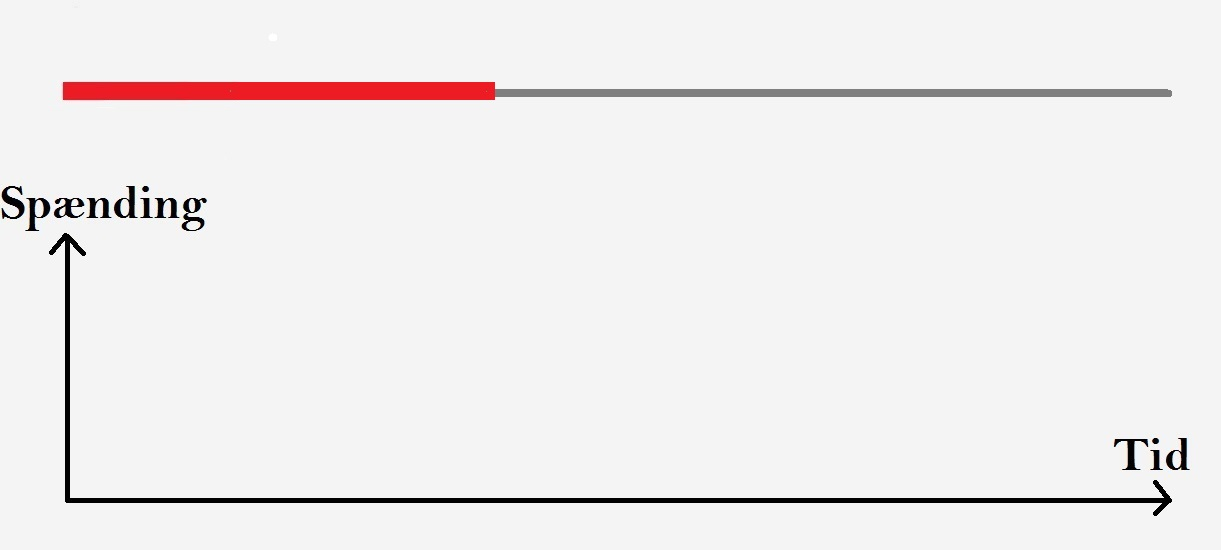
\includegraphics[width=4cm]{disposition/d12.jpg}
			\end{textblock*}
\end{frame}



\begin{frame}[t]
\frametitle{
		\LARGE{4. Gröbner-baser}}
			\begin{theorem}
				Lad $I \subseteq \K$ og $\leq$ være en ledordning. Da gælder
				\begin{enumerate}
					\item $I$ har en Gröbner-basis
					\item $I$ er endelig frembragt.
				\end{enumerate}						
			\end{theorem}				
			\begin{textblock*}{0.1cm}(8.78cm,7.78cm)  
				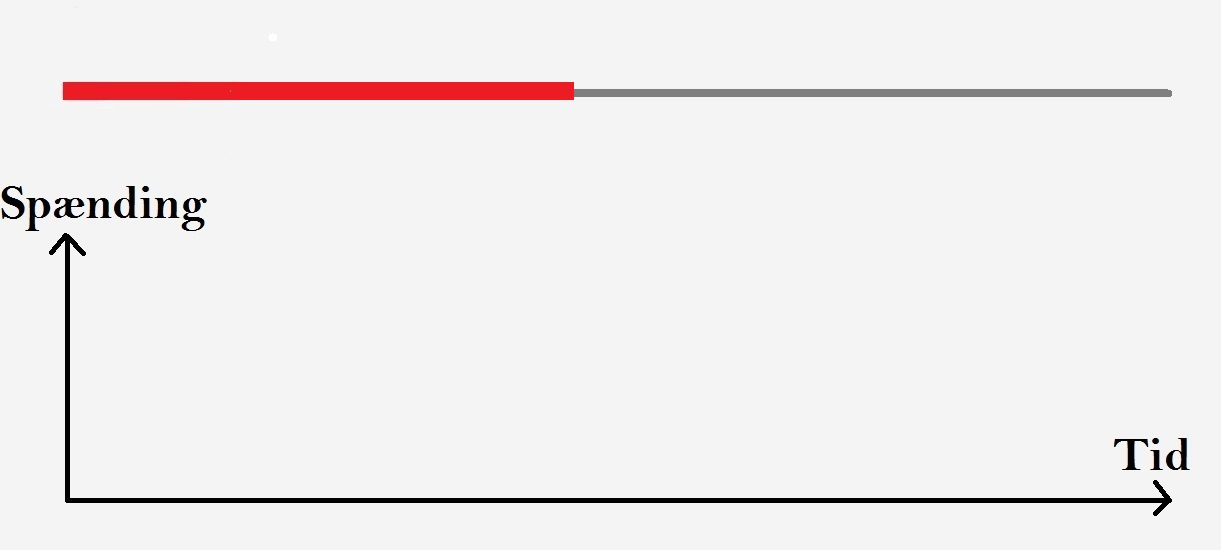
\includegraphics[width=4cm]{disposition/d13.jpg}
			\end{textblock*}
\end{frame}



\begin{frame}[t]
\frametitle{
		\LARGE{4. Gröbner-baser}}
			\visible<1->{\begin{theorem}
				Lad $I \subseteq \K$ og $\leq$ være en ledordning. Da gælder
				\begin{enumerate}
					\item $I$ har en Gröbner-basis
					\item $I$ er endelig frembragt. \bfseries{Hilberts basissætning}
				\end{enumerate}						
			\end{theorem}}
			\visible<2->{Beviset bruger \emph{Dicksons lemma}  }				
			\begin{textblock*}{0.1cm}(8.78cm,7.78cm)  
				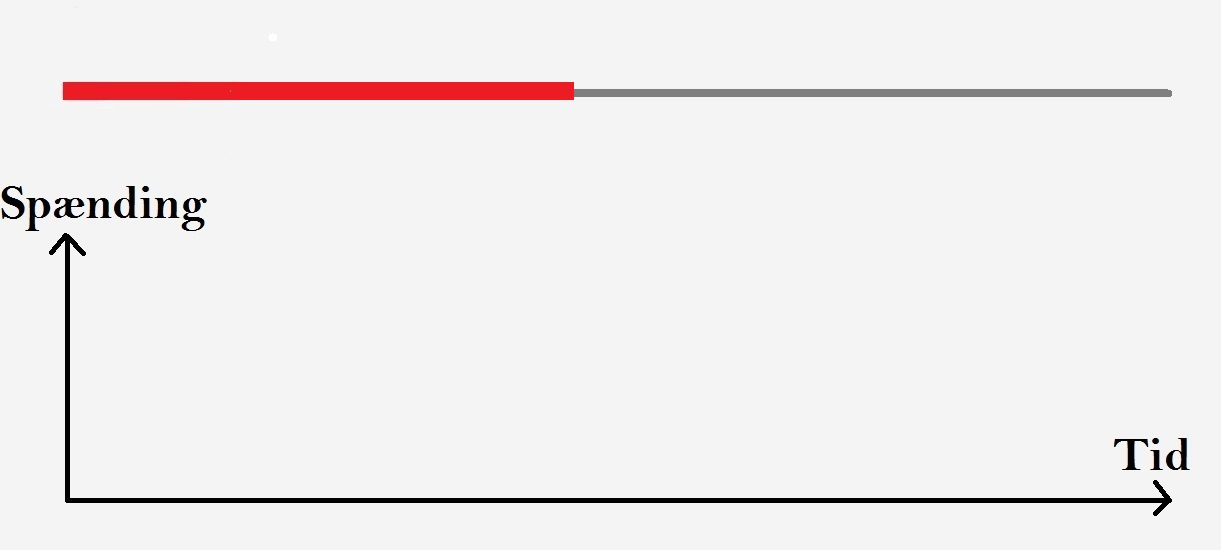
\includegraphics[width=4cm]{disposition/d13.jpg}
			\end{textblock*}
\end{frame}



\begin{frame}[t]
\frametitle{
		\LARGE{4. Gröbner-baser}}
			\visible<1->{\begin{definition}[\bfseries{Reducere til 0}]
			Lad $p \in \K$ og $P = \P \subseteq \K \setminus \{0\}$. Hvis der findes $a_1,\ldots ,a_m \in \K$ sådan, at
			\begin{enumerate}
				\item $p  =  a_1p_1 + \cdots + a_mp_m$ og
				\item $\IN(a_ip_i) \leq \IN(p)$,
			\end{enumerate}
			så siger vi
				\begin{align*}
					p \rightarrow_P 0.	
				\end{align*}
			\end{definition}}
			\visible<2->{Bemærk sammenhængen mellem $p^P = 0$ og $p \rightarrow_P 0$. }\\
			\visible<3->{Der gælder følgende sætning}
			\begin{textblock*}{0.1cm}(8.78cm,7.78cm)  
				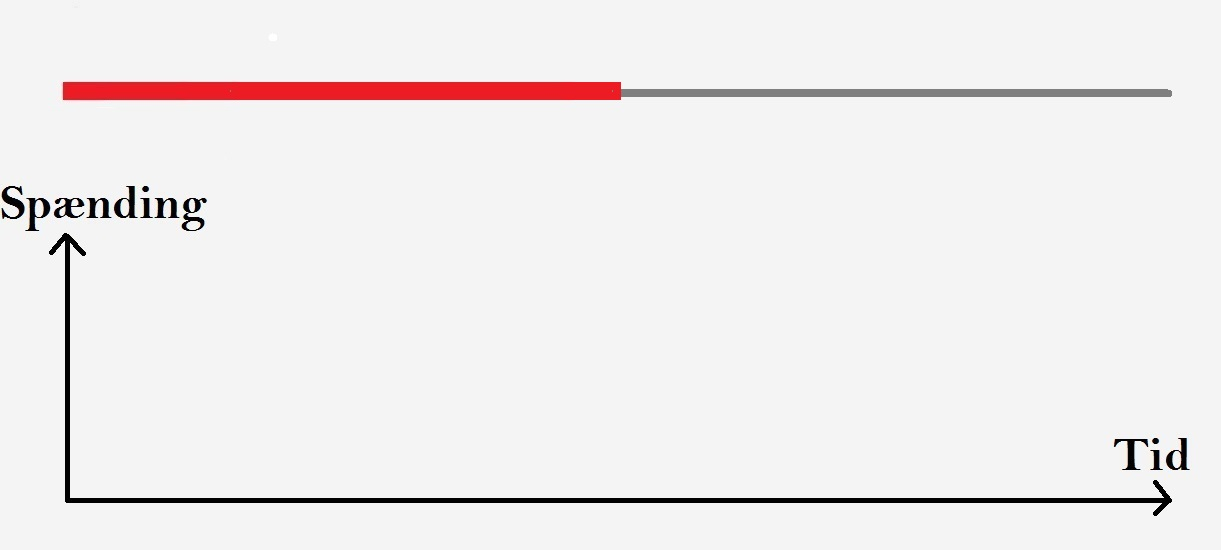
\includegraphics[width=4cm]{disposition/d13k.jpg}
			\end{textblock*}
\end{frame}



\begin{frame}[t]
\frametitle{
		\LARGE{4. Gröbner-baser}}
			\begin{theorem}
			\visible<1->{$P = \P$ og $I = \I$. Hvis der for alle $p \in I$ gælder, at $p \rightarrow_P 0$, \begin{bfseries} så er $P$ en Gröbner-basis for $I$\end{bfseries}.}  \\ \vspace{0.3cm}
			\visible<2->{Hvis $P$ er en Gröbner-basis for $I$, så gælder der for alle $p \in I$, at}
			\visible<2->{\begin{align*}
					p \rightarrow_P 0  \quad \Leftrightarrow \quad p^P = 0.
						\end{align*} }			
			\end{theorem}
			\begin{textblock*}{6cm}(1cm,5cm)
				\visible<3->{ Vi skal altså se på
				\begin{align*}
					p = a_1p_1 + \cdots + a_mp_m   \in I
				\end{align*}				 }
			\end{textblock*}
			\begin{textblock*}{6cm}(1cm,6.7cm)
				\visible<3->{ {\color{gray}Reducere til 0.}
					\begin{enumerate}
						\item ${\color{gray}p  =  a_1p_1 + \cdots + a_mp_m}${\color{gray} og}
						\item ${\color{gray}\IN(a_ip_i) \leq \IN(p)}$
					\end{enumerate}  }
			\end{textblock*}
			\begin{textblock*}{0.1cm}(8.78cm,7.78cm)  
				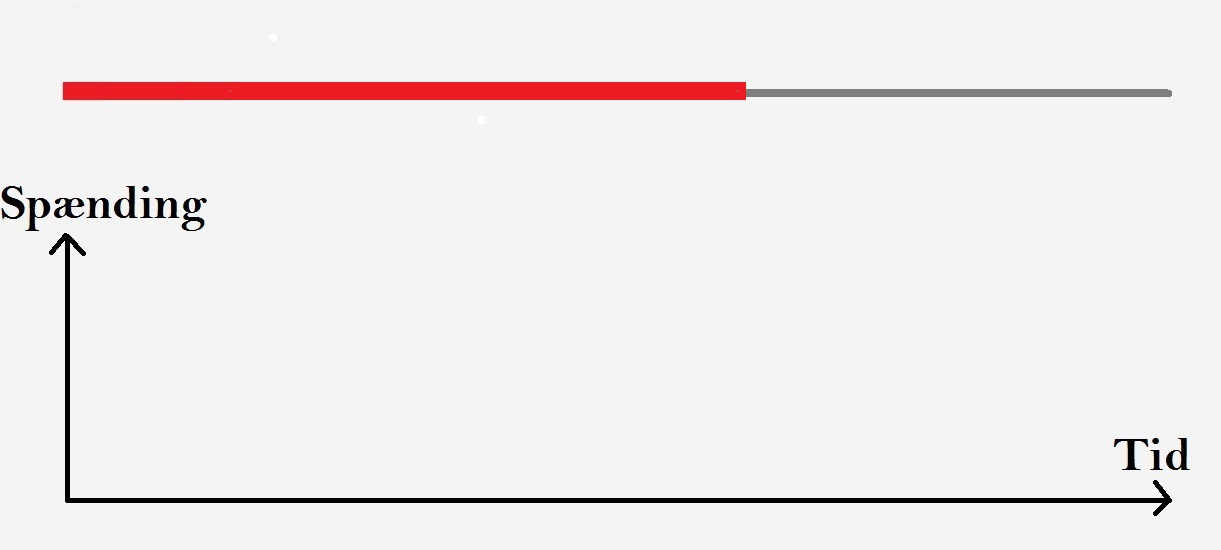
\includegraphics[width=4cm]{disposition/d14.jpg}
			\end{textblock*}
\end{frame}




\begin{frame}[t]
\frametitle{
		\LARGE{4. Gröbner-baser}}
		\visible<1->{Vi har brug for \emph{$S$-polynomiet} ! \\} 
		\visible<2->{\begin{definition}
						Sæt $\mathrm{mfm}\big(\IN(p),\IN(q)\big) := X^\xi$. Så er $S$-polynomiet af $p$ og $q$ mht. en ledordning $\leq$ givet ved
						\begin{align*}
							S(p,q)  =  X^{\xi}\bigg(\frac{p}{\IN(p)} - \frac{q}{\IN(q)}\bigg).
						\end{align*}
					\end{definition}  }
			\visible<3->{Eksempel \\ 
						Vi vil finde $S$-polynomiet af $p_1 = x^2+y^2+z^2-1$ og $p_2 = x+y+z$.}						
			\begin{textblock*}{0.1cm}(8.78cm,7.78cm)  
				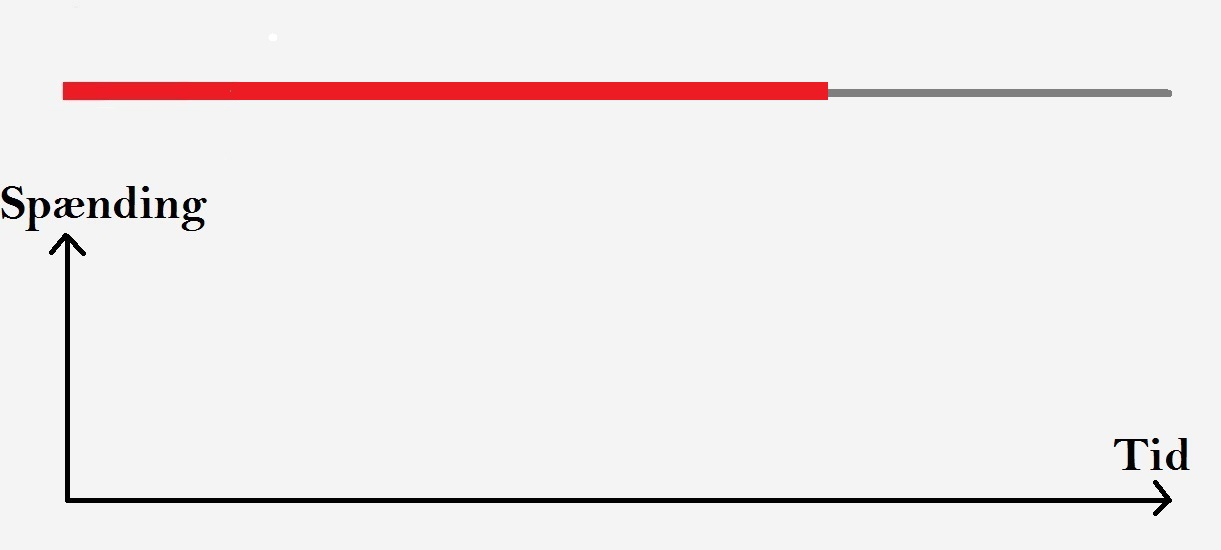
\includegraphics[width=4cm]{disposition/d15.jpg}
			\end{textblock*}
\end{frame}


\begin{frame}[t]
\frametitle{
		\LARGE{4. Gröbner-baser}}
\visible<1->{\begin{align*}
							S(p_1,p_2)    &=   \text{mfm}\big(\IN(p_1),\IN(p_2)\big) \bigg( \frac{p_1}{\IN(p_1)} - \frac{p_2}{\IN(p_2)} \bigg)  \\
										  &=  \text{mfm}(x^2,x)\bigg( \frac{x^2+y^2+z^2-1}{x^2}  -  \frac{x+y+z}{x} \bigg)  \\
										  &=  x^2\bigg( \frac{x^2+y^2+z^2-1}{x^2}  -  \frac{x+y+z}{x} \bigg)  \\
										  &=  x^2+y^2+z^2-1 - x^2-xy-xz  \\
										  &=  -xy -xz +y^2 +z^2 -1  
\end{align*} }
				\begin{textblock*}{0.1cm}(8.78cm,7.78cm)  
					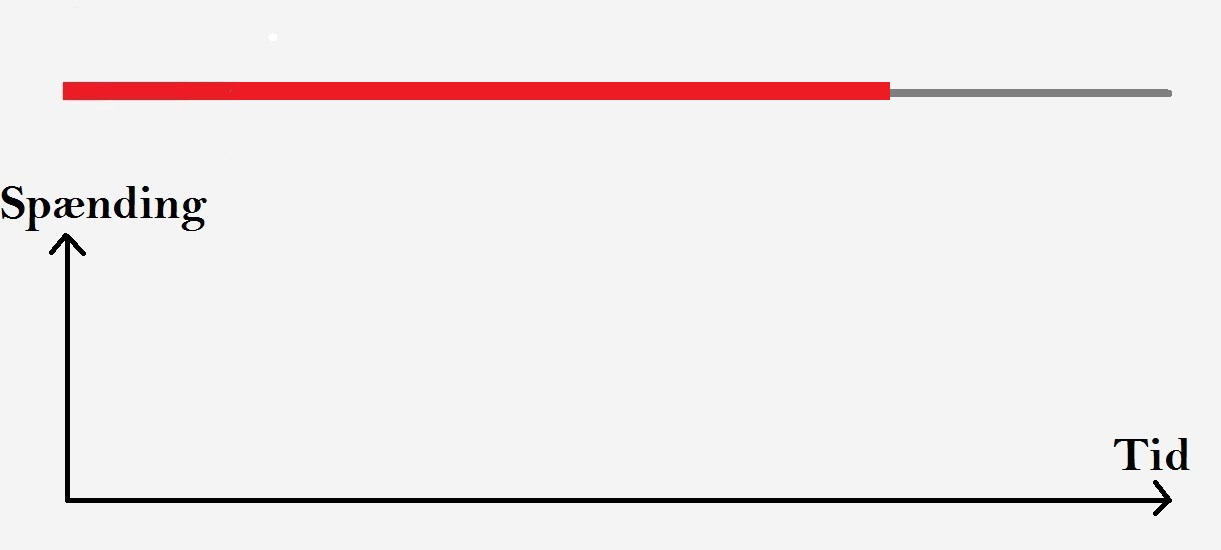
\includegraphics[width=4cm]{disposition/d16.jpg}
				\end{textblock*}
\end{frame}



\begin{frame}[t]
\frametitle{
		\LARGE{4. Gröbner-baser}}
				\begin{textblock*}{0.1cm}(8.78cm,7.78cm)  
					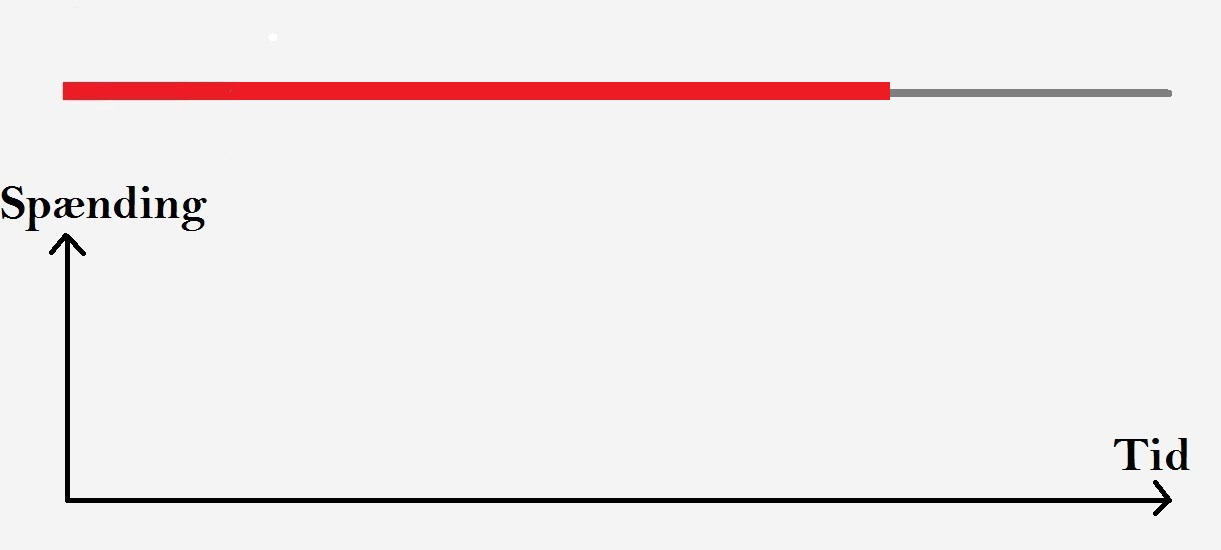
\includegraphics[width=4cm]{disposition/d16.jpg}
				\end{textblock*}				
				\begin{textblock*}{0.85cm}(1cm,0cm)
					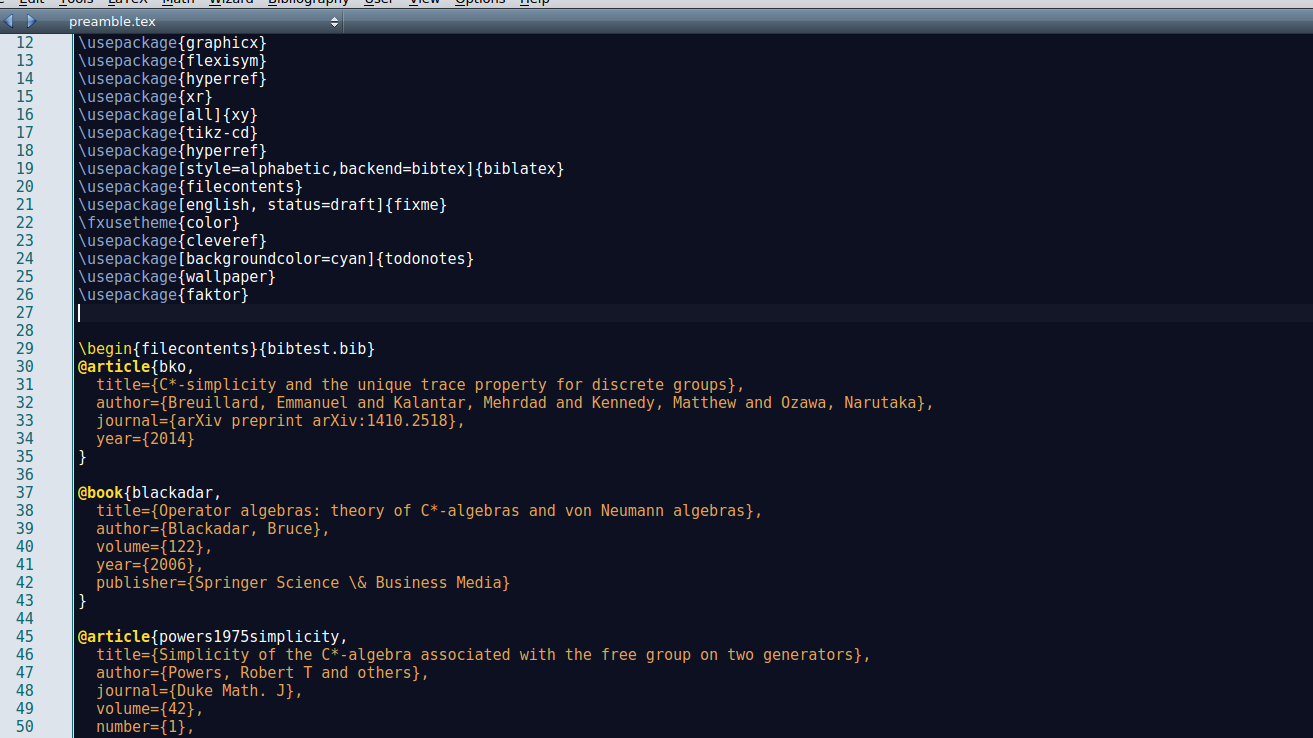
\includegraphics[scale=0.087]{1.jpg}
				\end{textblock*}				
\end{frame}


\begin{frame}[t]
\frametitle{
		\LARGE{4. Gröbner-baser}}
				\begin{textblock*}{0.1cm}(8.78cm,7.78cm)  
					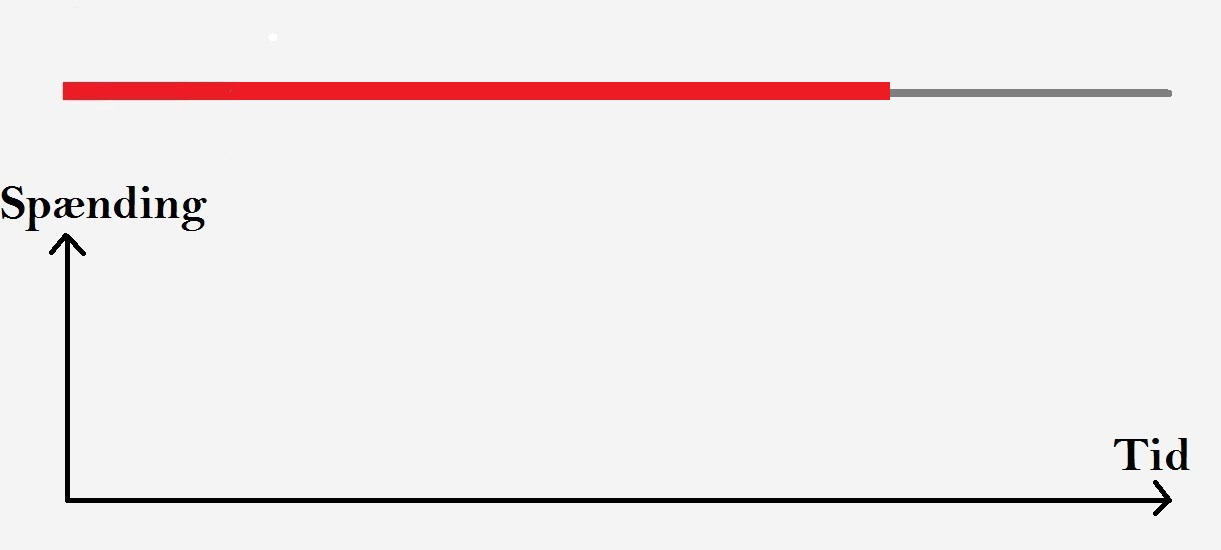
\includegraphics[width=4cm]{disposition/d16.jpg}
				\end{textblock*}				
				\begin{textblock*}{0.85cm}(1cm,0cm)
					
\includegraphics[scale=0.087]{2.jpg}
				\end{textblock*}				
\end{frame}

\begin{frame}[t]
\frametitle{
		\LARGE{4. Gröbner-baser}}
				\begin{textblock*}{0.1cm}(8.78cm,7.78cm)  
					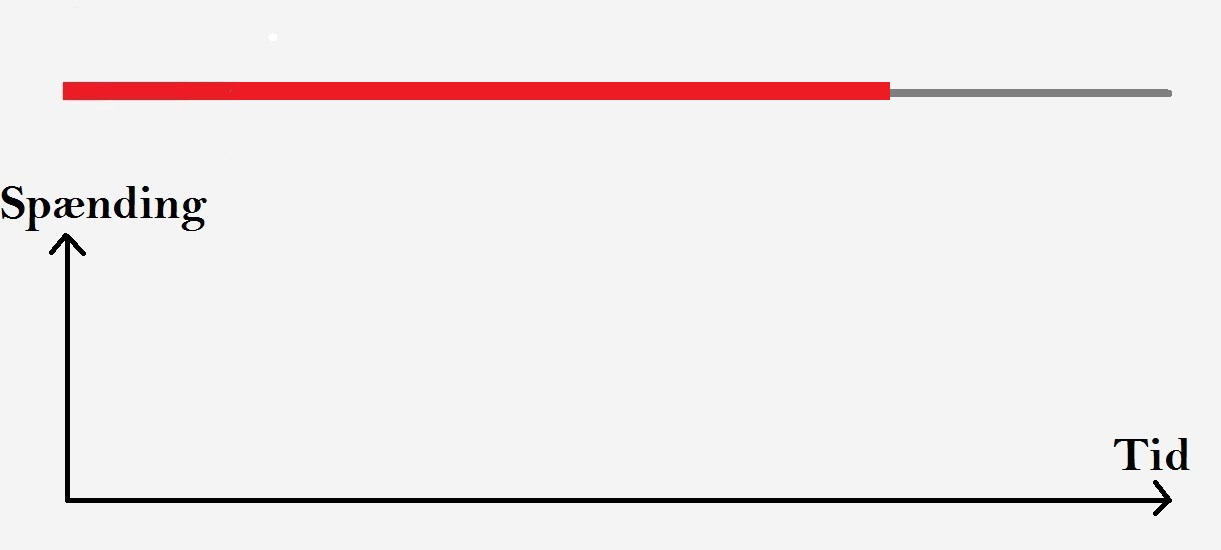
\includegraphics[width=4cm]{disposition/d16.jpg}
				\end{textblock*}				
				\begin{textblock*}{0.85cm}(1cm,0cm)
					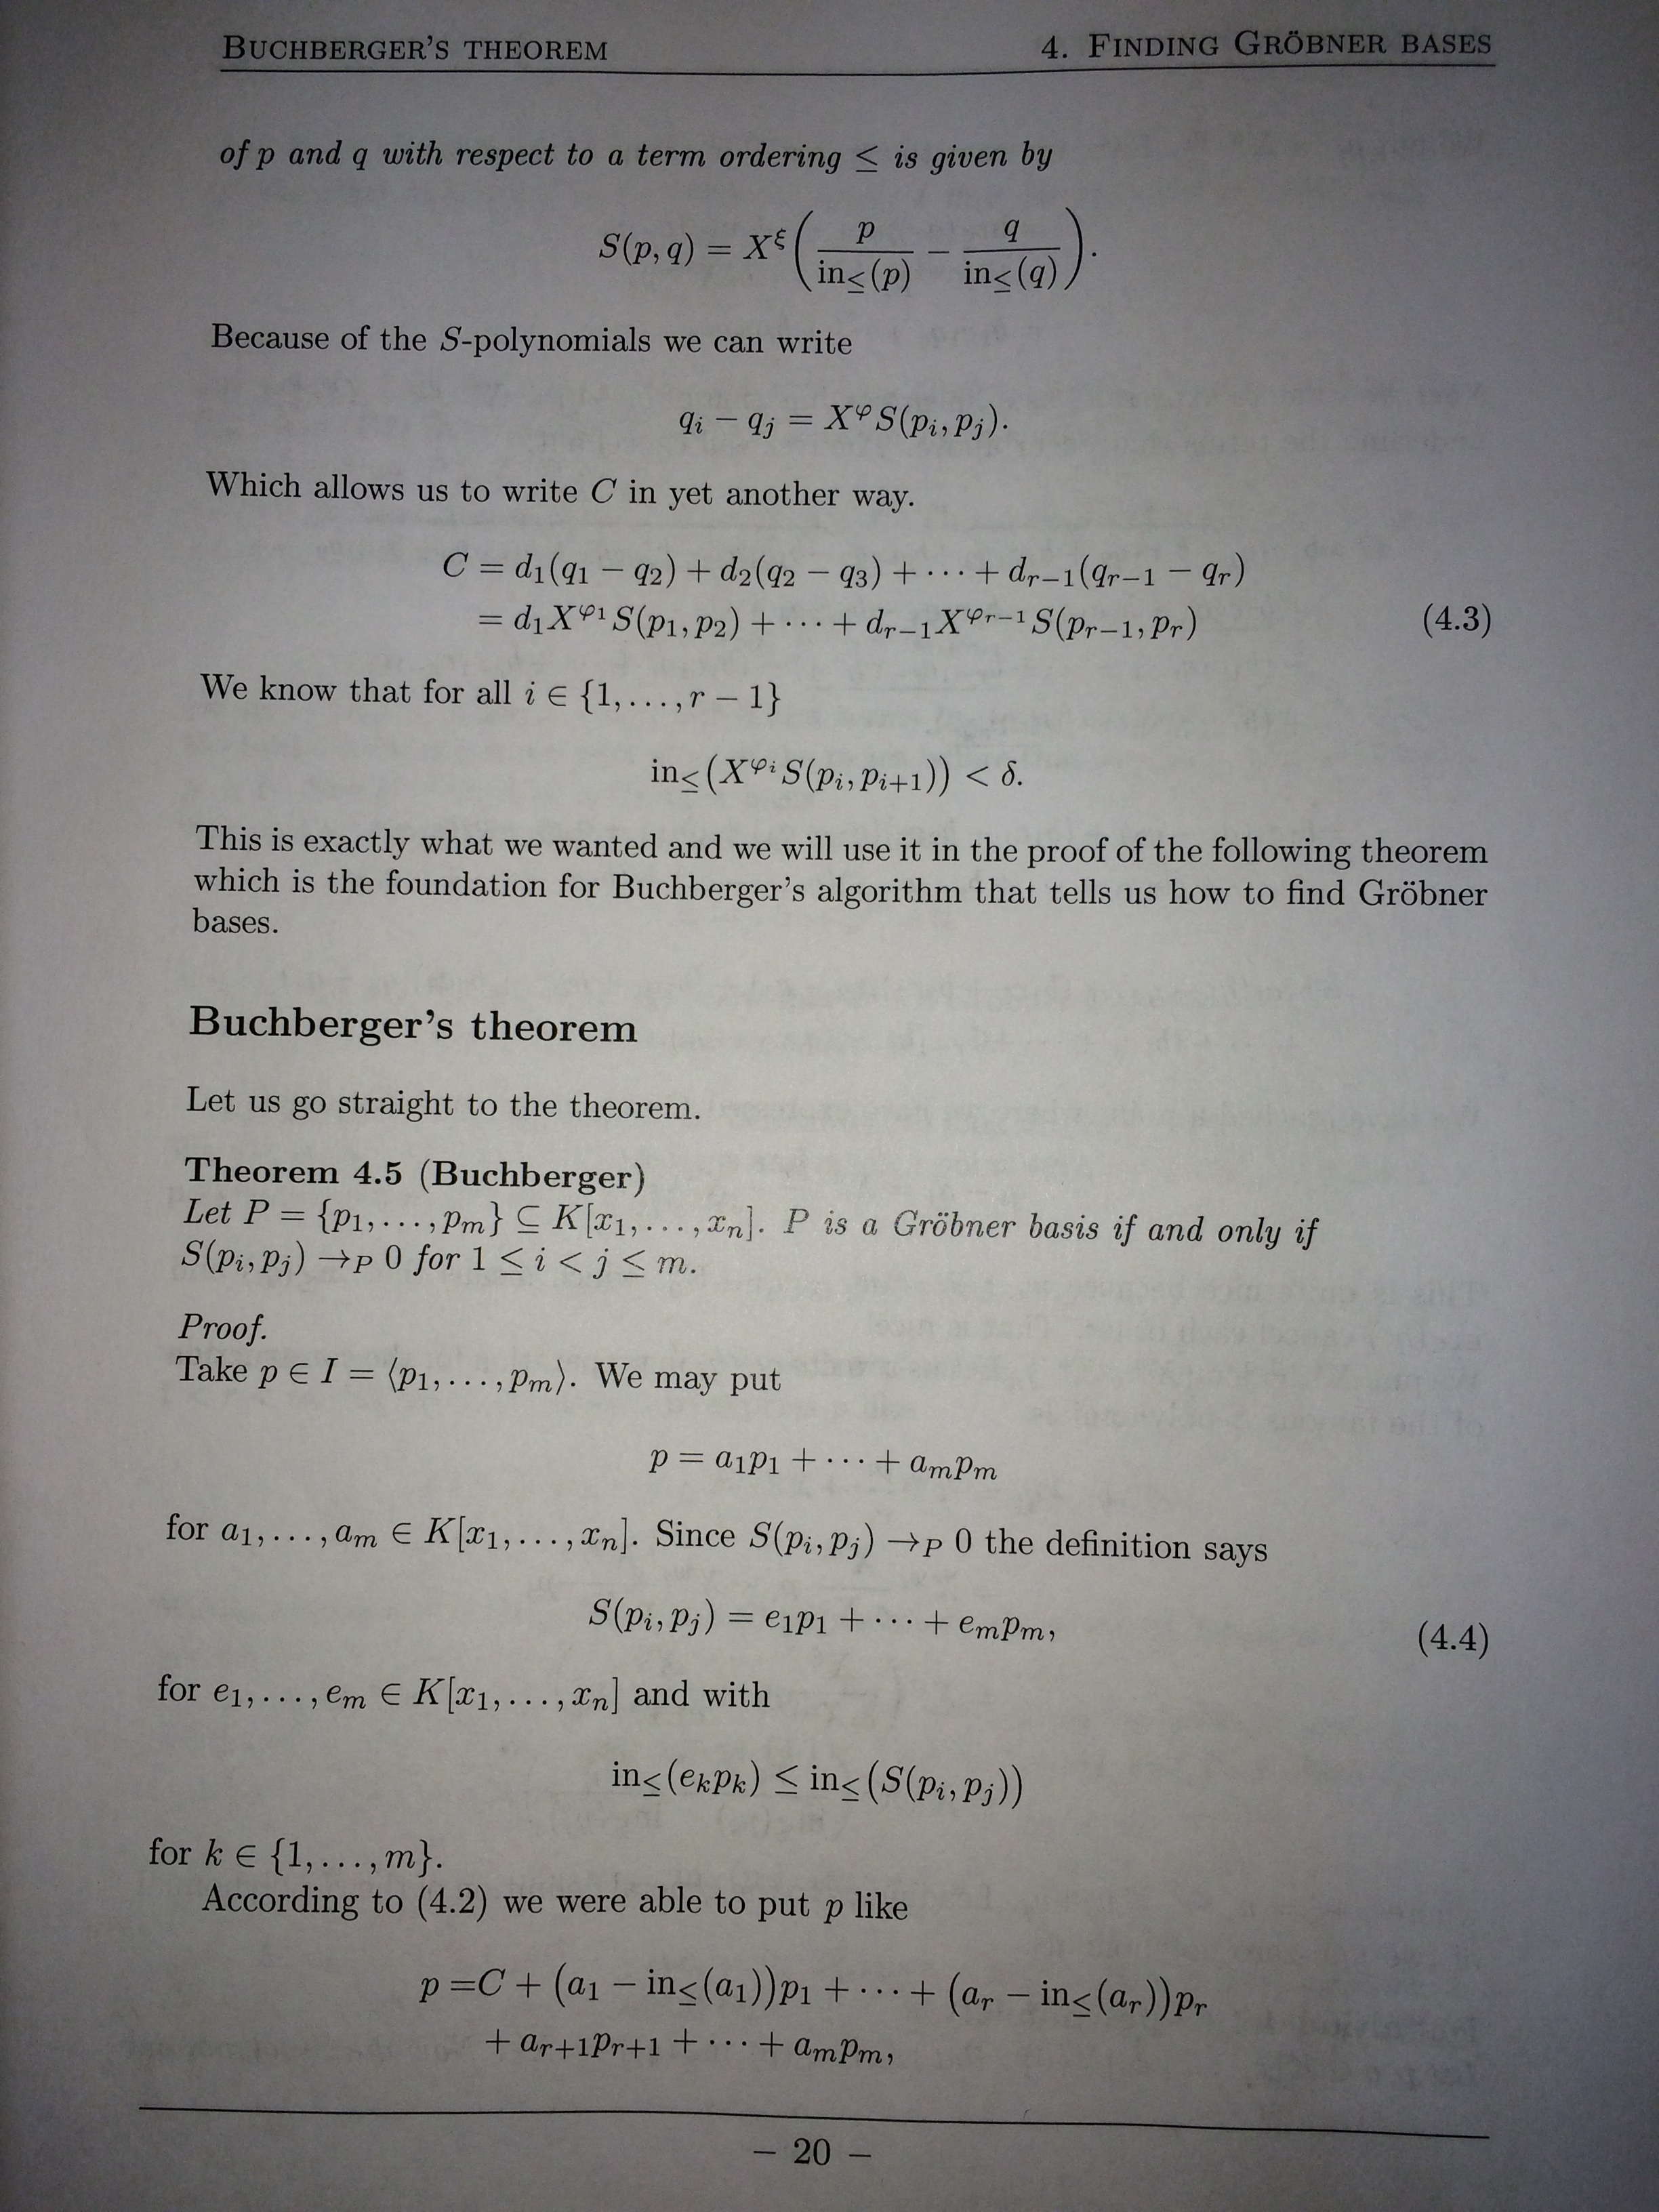
\includegraphics[scale=0.087]{3.jpg}
				\end{textblock*}				
\end{frame}






\begin{frame}[t]
\frametitle{
		\LARGE{4. Gröbner-baser}}
				\begin{theorem}[\bfseries{Buchbergers sætning}]
					Lad $P = \P$. $P$ er en Gröbner-basis hvis og kun hvis der for $1\leq i < j \leq m$ gælder, at $S(p_i,p_j)\rightarrow_P 0$.
				\end{theorem}								\vspace*{0.2cm}
				\visible<2->{Beviset bruger netop den lækre egenskab ved $S$-polynomiet.}\vspace*{0.2cm}
				\visible<3->{Sammenhængen mellem $p\rightarrow_P 0$ og $p^P = 0$ giver os $S$-kriteriet:} \vspace*{0.2cm}
				\visible<3->{ \begin{theorem}[\bfseries{S-kriteriet}]
					Lad $P = \P$. $P$ er en Gröbner-basis hvis og kun hvis der for $1\leq i < j \leq m$ gælder, at $S(p_i,p_j)^P = 0$.
				\end{theorem}								 }
				\begin{textblock*}{0.1cm}(8.78cm,7.78cm)  
					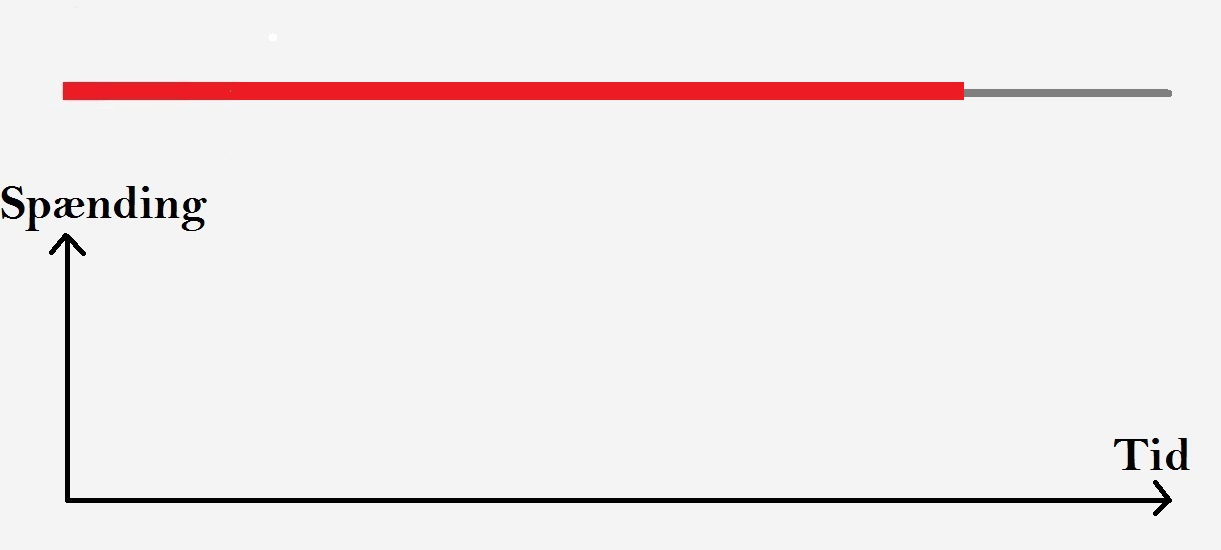
\includegraphics[width=4cm]{disposition/d17.jpg}
				\end{textblock*}	
\end{frame}




\begin{frame}[t]
\frametitle{
		\LARGE{4. Gröbner-baser}}
				\begin{bfseries} Buchbergers algoritme\end{bfseries} \\
					 $P = \P$. Finder $p_k$ og $p_l$, så $S(p_k,p_l)^P \neq 0$.\\ \vspace*{0.1cm}
					 \visible<2->{Så tilføjer vi  $S(p_k,p_l)^P$ til mængden af polynomier og får }
					 \visible<2->{\begin{align*}
							P'  =  P \cup \{S(p_k,p_l)^P\}  =  \{p_1,\ldots ,p_m, S(p_k,p_l)^P\}.	 
						 \end{align*} }
					 \visible<3->{Finder $p_r,p_s \in P'$, så  $S(p_r,p_s)^{P'}  \neq  0$. } \\ \vspace*{0.1cm}
					 \visible<4->{Vi tilføjer blot}
					 \visible<5->{\begin{align*}
		P''  =  P' \cup  \{ S(p_r,p_s)^{P'} \}  =  \{  p_1,\ldots ,p_m, S(p_k,p_l)^P, S(p_r,p_s)^{P'} \}
	\end{align*} }
					\visible<6->{\emph{Stopper det på et tidspunkt?}} \\ \vspace*{0.1cm}
					\visible<7->{\begin{bfseries}Ja! Dicksons lemma sikrer os endnu en gang\end{bfseries}.}
				\begin{textblock*}{0.1cm}(8.78cm,7.78cm)  
					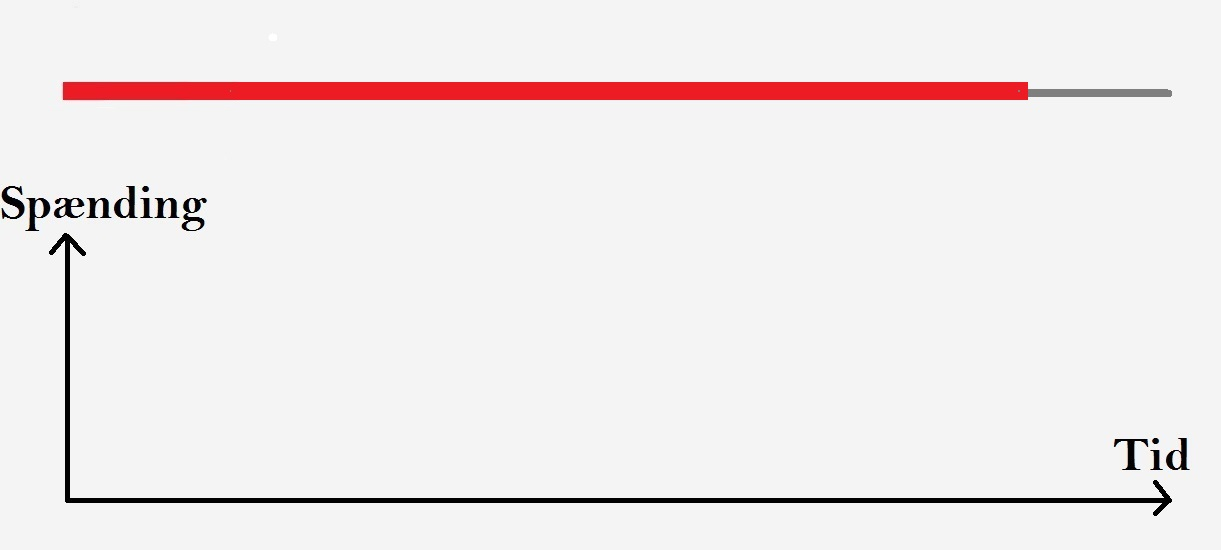
\includegraphics[width=4cm]{disposition/d18.jpg}
				\end{textblock*}	
\end{frame}



\begin{frame}[t]
\frametitle{
		\LARGE{4. Gröbner-baser}}
					Vi er \emph{altid} i stand til at finde Gröbner-basen for et ideal! \\  \vspace*{1cm}
					\visible<2->{\begin{bfseries}\emph{Kan det bruges til noget?}\end{bfseries} }
				\begin{textblock*}{0.1cm}(8.78cm,7.78cm)  
					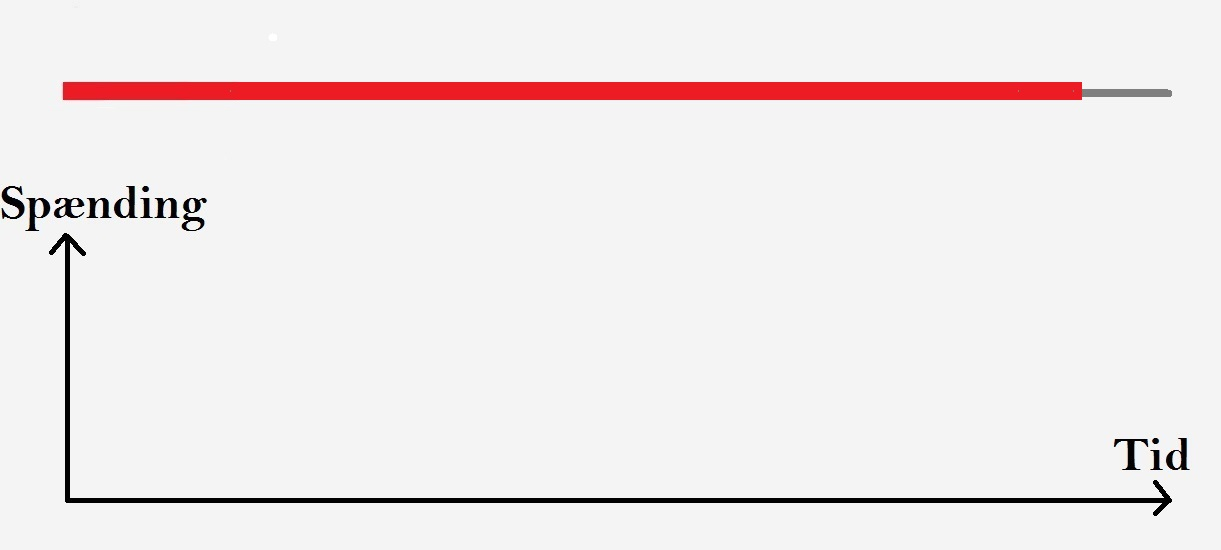
\includegraphics[width=4cm]{disposition/d19.jpg}
				\end{textblock*}	
\end{frame}













\begin{frame}[t]
\frametitle{
		\LARGE{5. Anvendelser}}
					\begin{itemize}
					\item Robotvidenskab
					\item Generel optimering
					\end{itemize} 
					\visible<2->{\vspace*{0.5cm} \begin{table}
\begin{tabular}{|c|c||c|c|} 
\hline
 &  &  & 4\\
\hline
4 &  & 2 & \\
\hline\hline
 & 3 &  & 1\\
\hline
 &  &  & \\
\hline
\end{tabular}
\end{table}  }
				\begin{textblock*}{0.1cm}(8.78cm,7.78cm)  
					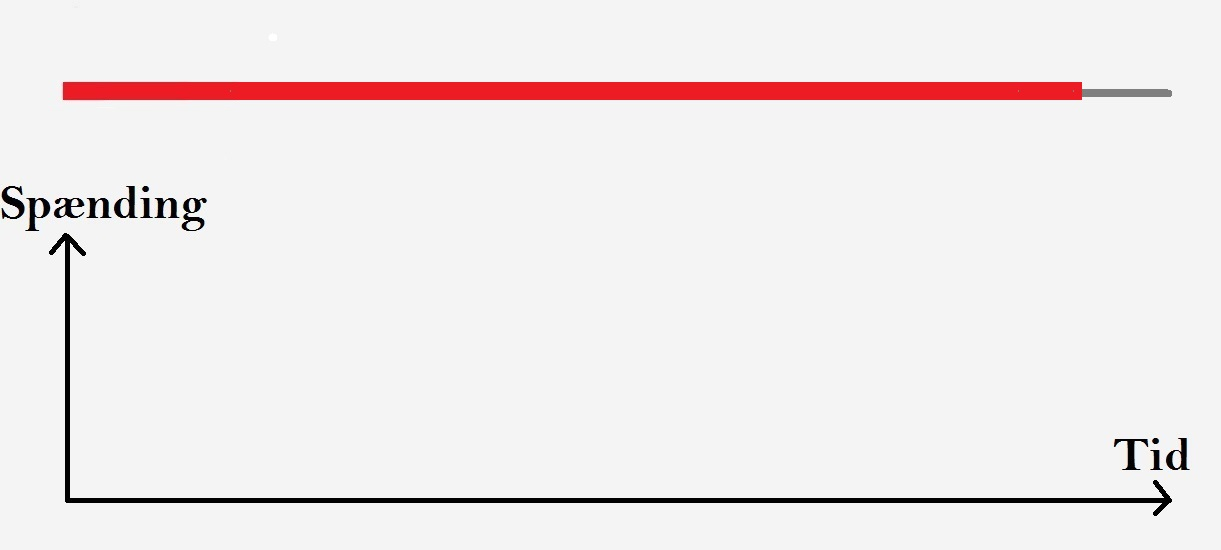
\includegraphics[width=4cm]{disposition/d19.jpg}
				\end{textblock*}	
\end{frame}



\begin{frame}[t]
\frametitle{
		\LARGE{5. Anvendelser}}
\begin{textblock*}{5cm}(7cm,0.5cm)
\begin{table} 
\begin{tabular}{|c|c||c|c|} 
\hline
${\color{blue}x_1}$ & $x_2$ & $x_3$ & $x_4$\\
\hline
$x_5$ & $x_6$ & $x_7$ & $x_8$ \\
\hline\hline
$x_9$ & $x_{10}$ & $x_{11}$ & $x_{12}$\\
\hline
$x_{13}$ & $x_{14}$ & $x_{15}$ & $x_{16}$\\
\hline
\end{tabular} 
\end{table}
\end{textblock*}
\begin{textblock*}{0.1cm}(1cm,1cm)
\visible<2->{\begin{align*}
{\color{blue}(x_1-1)(x_1-2)(x_1-3)(x_1-4)} &= 0  \\
  &\vdots \\
(x_{16}-1)(x_{16}-2)(x_{16}-3)(x_{16}-4) &= 0.   
\end{align*}}
\end{textblock*}
				\begin{textblock*}{0.1cm}(8.78cm,7.78cm)  
					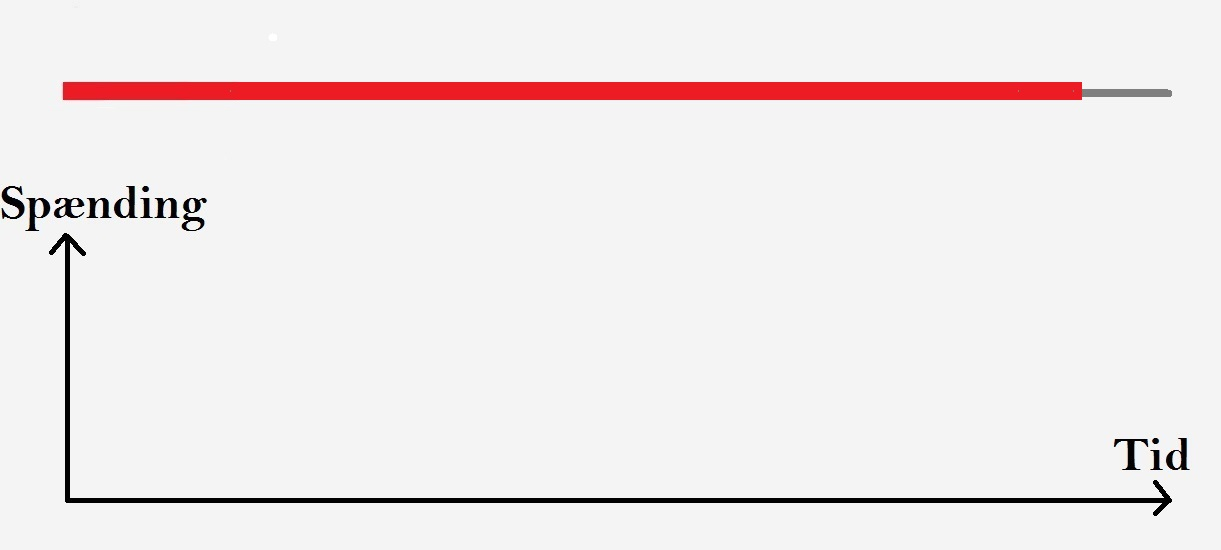
\includegraphics[width=4cm]{disposition/d19.jpg}
				\end{textblock*}	
\end{frame}



\begin{frame}[t]
\frametitle{
		\LARGE{5. Anvendelser}}
\begin{textblock*}{5cm}(7cm,0.5cm)
\begin{table} 
\begin{tabular}{|c|c||c|c|} 
\hline
${\color{blue}x_1}$ & ${\color{blue}x_2}$ & ${\color{blue}x_3}$ & ${\color{blue}x_4}$\\
\hline
$x_5$ & $x_6$ & $x_7$ & $x_8$ \\
\hline\hline
$x_9$ & $x_{10}$ & ${\color{red}x_{11}}$ & ${\color{red}x_{12}}$\\
\hline
$x_{13}$ & $x_{14}$ & ${\color{red}x_{15}}$ & ${\color{red}x_{16}}$\\
\hline
\end{tabular} 
\end{table}
\end{textblock*}
\begin{textblock*}{0.1cm}(1cm,1cm)
\begin{align*}
(x_1-1)(x_1-2)(x_1-3)(x_1-4) &= 0  \\
  &\vdots \\
(x_{16}-1)(x_{16}-2)(x_{16}-3)(x_{16}-4) &= 0\\
{\color{blue}x_1x_2x_3x_4 - 24} &= 0  \\
   &\vdots  \\
{\color{red}x_{11}x_{12}x_{15}x_{16} - 24} &= 0. 
\end{align*}
\end{textblock*}
				\begin{textblock*}{0.1cm}(8.78cm,7.78cm)  
					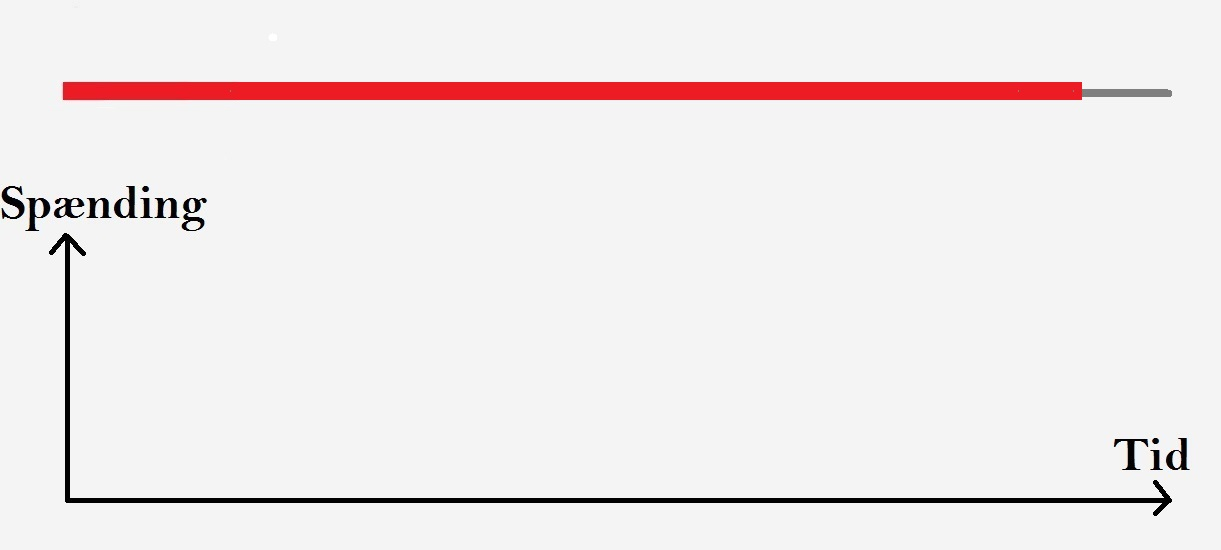
\includegraphics[width=4cm]{disposition/d19.jpg}
				\end{textblock*}	
\end{frame}


\begin{frame}[t]
\frametitle{
		\LARGE{5. Anvendelser}}
\begin{textblock*}{5cm}(7cm,0.5cm)
\begin{table} 
\begin{tabular}{|c|c||c|c|} 
\hline
${\color{blue}x_1}$ & ${\color{blue}x_2}$ & ${\color{blue}x_3}$ & ${\color{blue}x_4}$\\
\hline
$x_5$ & $x_6$ & $x_7$ & $x_8$ \\
\hline\hline
$x_9$ & $x_{10}$ & $x_{11}$ & $x_{12}$\\
\hline
$x_{13}$ & $x_{14}$ & $x_{15}$ & $x_{16}$\\
\hline
\end{tabular} 
\end{table}
\end{textblock*}
\begin{textblock*}{0.1cm}(1cm,1cm)
\begin{align*}
(x_1-1)(x_1-2)(x_1-3)(x_1-4) &= 0  \\
  &\vdots \\
(x_{16}-1)(x_{16}-2)(x_{16}-3)(x_{16}-4) &= 0\\
x_1x_2x_3x_4 - 24 &= 0  \\
   &\vdots  \\
x_{11}x_{12}x_{15}x_{16} - 24 &= 0 \\
{\color{blue}x_1 + x_2 + x_3 + x_4 - 10} &= 0  \\
  &\vdots  \\
 x_{11} + x_{12} + x_{15} + x_{16} - 10 &= 0. \\
\end{align*}
\end{textblock*}
\begin{textblock*}{5cm}(2cm,8cm)
40 ligninger.
\end{textblock*}
				\begin{textblock*}{0.1cm}(8.78cm,7.78cm)  
					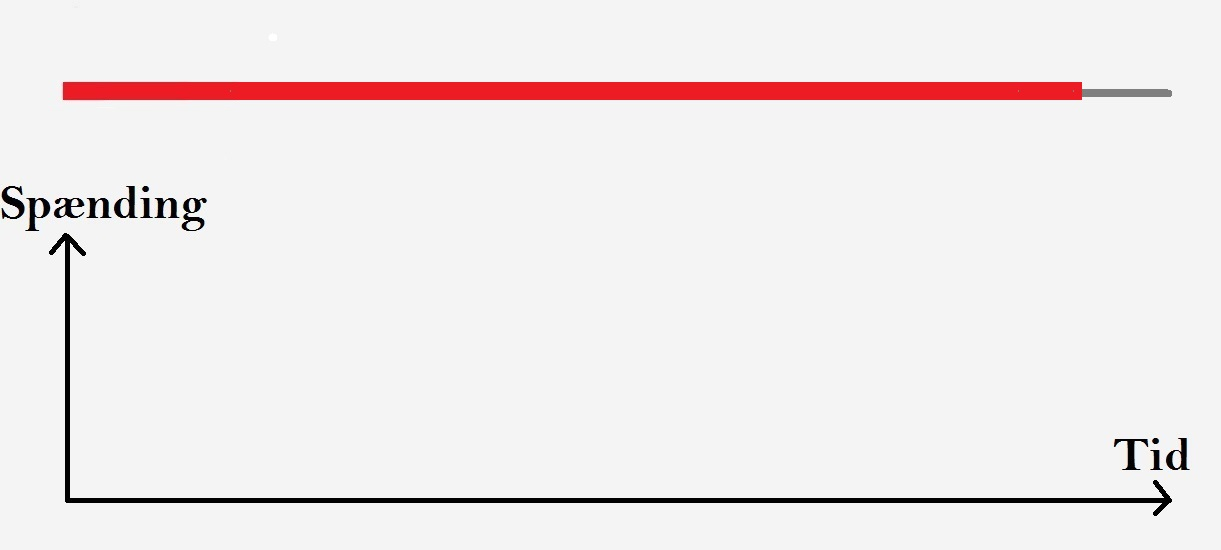
\includegraphics[width=4cm]{disposition/d19.jpg}
				\end{textblock*}	
\end{frame}




\begin{frame}[t]
\frametitle{
		\LARGE{5. Anvendelser}}
\begin{table}
\begin{tabular}{|c|c||c|c|} 
\hline
 &  &  & 4\\
\hline
4 &  & 2 & \\
\hline\hline
 & 3 &  & 1\\
\hline
 &  &  & \\
\hline
\end{tabular}
\end{table} 
De 40 ligninger sammen med:
\begin{align*}
	x_4 - 4 &= 0 \\
	x_5 - 4 &= 0 \\
	x_7 - 2 &= 0 \\
	x_{10} - 3 &= 0 \\
	x_{12} - 1 &= 0
\end{align*}

				\begin{textblock*}{0.1cm}(8.78cm,7.78cm)  
					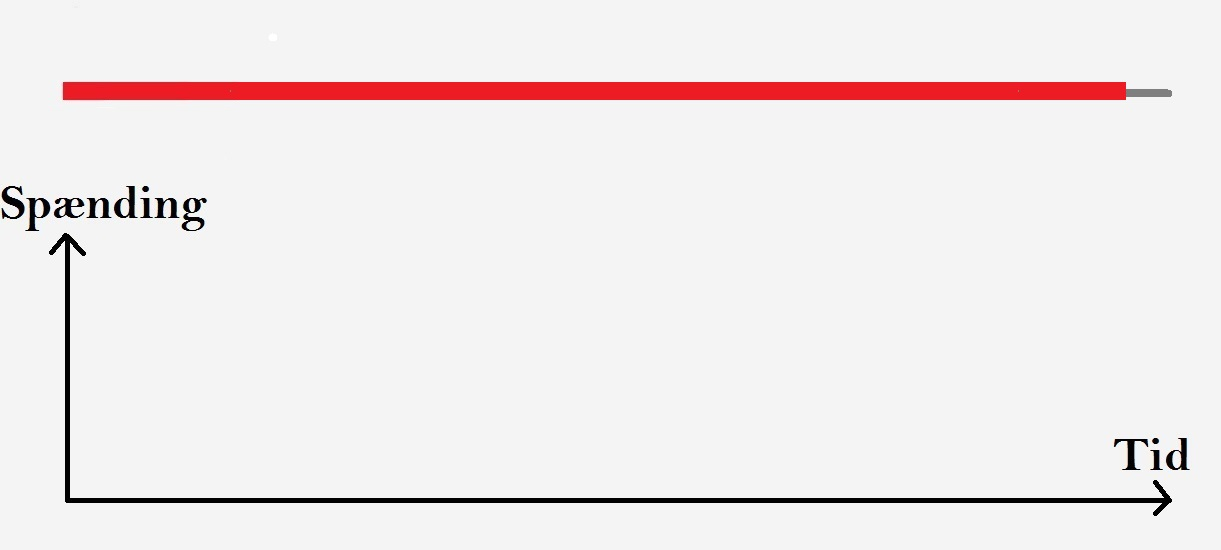
\includegraphics[width=4cm]{disposition/d20.jpg}
				\end{textblock*}	
\end{frame}


\begin{frame}[t]
\frametitle{
		\LARGE{5. Anvendelser}}
Vi finder Gröbner-basen for idealet frembragt af de 45 ligninger vha. en computer og får et nyt ligningssystem.
\begin{table}
\begin{tabular}{c c} 

$x_{1}-3 = 0$ & $x_{2}-2 = 0$ \\

$x_{3}-1 = 0$ & ${\color{blue}x_{4}-4 = 0}$ \\

${\color{blue}x_{5}-4 = 0}$  & $x_{6}-1 = 0$\\

${\color{blue}x_{7}-2 = 0}$ & $x_{8}-3 = 0$ \\

$x_{9}-2 = 0$ & ${\color{blue}x_{10}-3 = 0}$ \\

$x_{11}-4 = 0$ & ${\color{blue}x_{12}-1 = 0}$ \\

$x_{13}-1 = 0$ & $x_{14}-4 = 0$ \\

$x_{15}-3 = 0$ & $x_{16}-2 = 0$.

\end{tabular}
\end{table} 

				\begin{textblock*}{0.1cm}(8.78cm,7.78cm)  
					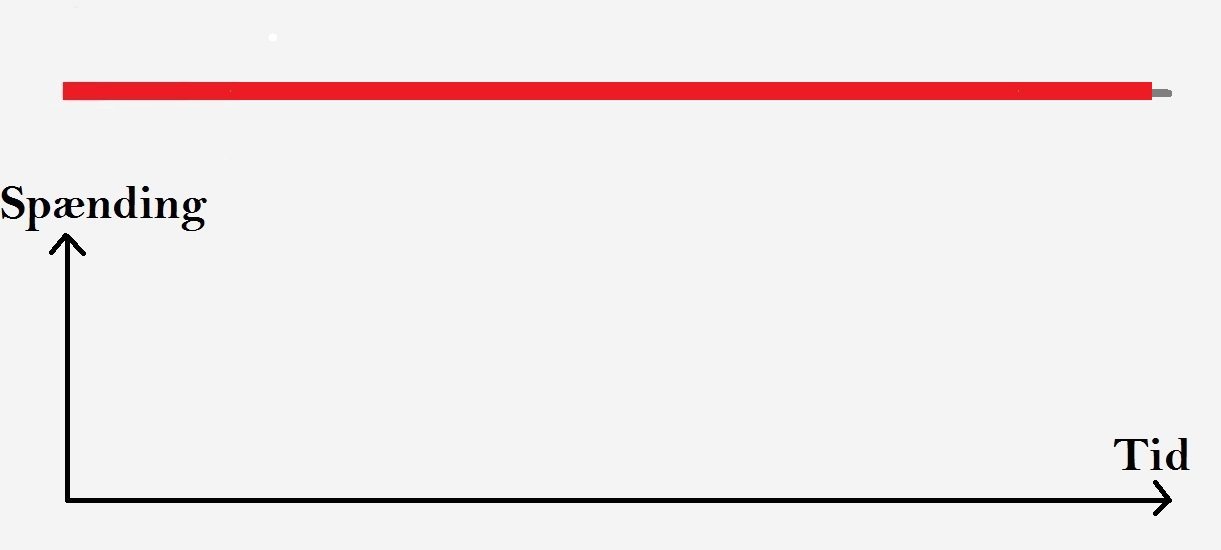
\includegraphics[width=4cm]{disposition/d21.jpg}
				\end{textblock*}	
\end{frame}









\begin{frame}[t]
\frametitle{
		\LARGE{6. Lyn-opsummering}}

				\begin{textblock*}{0.1cm}(8.78cm,7.78cm)  
					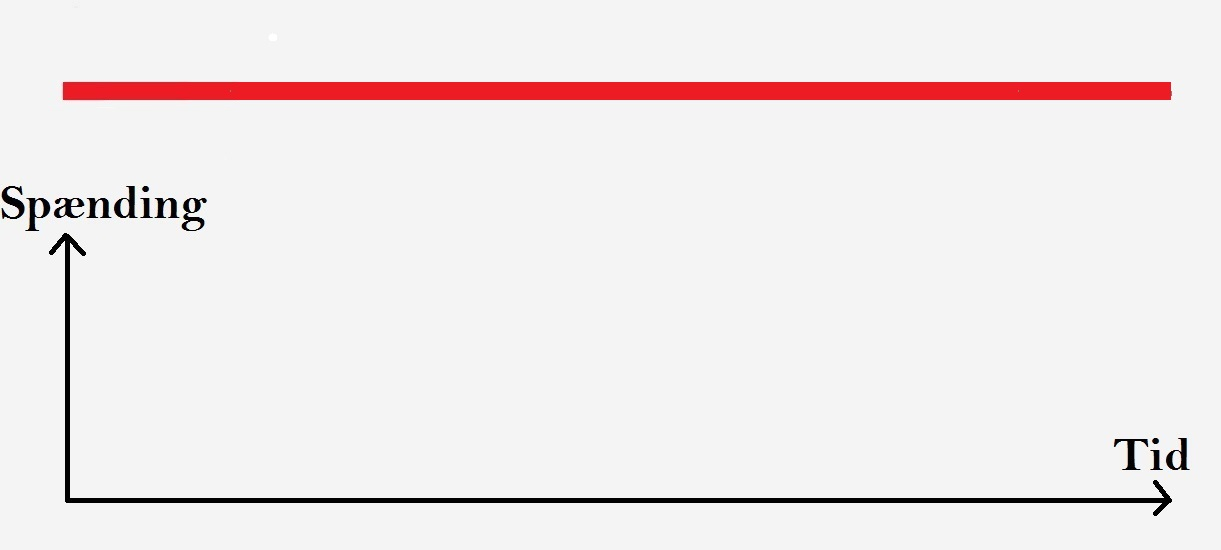
\includegraphics[width=4cm]{disposition/d22.jpg}
				\end{textblock*}	
\end{frame}




\end{document}